% Выбор класса документа
%\documentclass {book}
%\documentclass {article}
\documentclass [a4paper, 12pt, oneside]{scrbook}
% Чтобы можно было использовать русские буквы в формулах,
%но в случае использования предупреждать об этом
\usepackage [warn]{mathtext}
% Выбор внутренней TEX−кодировки
\usepackage[T2A]{fontenc}
% Выбор кодовой страницы документа
% Так же можно выбрать cp1251 или utf8
\usepackage[utf8]{inputenc}
% Выбор языка документа
\usepackage[english,russian]{babel}
% Начинать первый параграф
\usepackage{indentfirst}

% Загрузка пакета hyperref
\usepackage[unicode=true] {hyperref}
%\usepackage{url}
\usepackage{colortbl}
\usepackage{tabularx}

\usepackage{graphicx}
\graphicspath{pictures/}
\DeclareGraphicsExtensions{.pdf,.png,.jpg}

%\makeatletter
%\renewcommand*{\@biblabel}[1]{\hfill#1.}
%\makeatother

%\usepackage[backend=biber]{biblatex}
%\addbibresource{references.bib}

%установка тире для подрисуночной подписи
\RequirePackage{caption}
\DeclareCaptionLabelSeparator{defffis}{ --- }
\captionsetup{justification=centering,labelsep=defffis}

\usepackage{csquotes}
\usepackage{debate}
\usepackage[nopygments,nonumbers,noframes]{ffcode}
\usepackage{to-be-determined}
\usepackage{inputenc}

\newcommand\code[1]{\ff{#1}}

% Конец преамбулы и начало документа
\begin {document}

% Изменение начала подрисуночной надписи
\renewcommand\figurename{Рисунок}

% --- Титульная страница -----------------------------------

\title{\Huge{Архитектура вычислительных систем\\ \large{Учебное пособие}}}

\author {{\Large{А.\,И.~Легалов}}
\and {\Large{С.\,А.~Виденин}}}

%\date {13.08.2022}
\maketitle

% --- Оглавление -------------------------------------------

\tableofcontents

% Основная часть
%\mainmatter

% --- Введение -------------------------------------------
% Введение

\chapter* {Введение}
\addcontentsline{toc}{chapter}{Введение}

Вычислительные системы (ВС) различного назначения в настоящее время используются практически повсеместно. Они сопровождают нас в повседневной жизни, используются в промышленности и в быту, поддерживают игровой контент и решение экономических проблем. Несмотря на их разнообразие существуют некоторые общие принципы, связанные с особенностями организации и построения вычислительных систем, которые необходимо знать для повышения эффективности их использования. Эти принципы отражаются в архитектурных решениях, обеспечивающих представление как внутренней структуры ВС так и их взаимодействия с пользователями, которыми в большинстве своем являются программистами.

\section*{Цель и задачи}

Целью дисциплины является изучение особенностей архитектур вычислительных систем, их многоуровневости и разнообразия. Для достижения поставленной цели предполагается рассмотреть следующие основные разделы:

\begin{itemize}
 \item Общее понятие архитектуры ВС. Классификация архитектур ВС
 \item Особенности архитектуры ВС уровня системы команд.
 \item Отображение архитектуры ВС уровня системы команд в языках системного программирования и ассемблере.
 \item Уровень операционной системы и его использование в низкоуровневом программировании.
 \item Разнообразие архитектур уровня системы команд.
 \item Поддержка архитектуры уровня системы команд на уровне микроархитектур.
 \item Отображение параллелизма в архитектурах ВС.
\end{itemize}


\section*{Основные темы, затрагиваемые при изучении дисциплины}

При всей многоуровневости и разнообразии архитектур ВС рамках изучаемой дисциплины основной упор предполагается сделать на уровень системы команд и параллелизм. Это обуславливается тем, что в объеме одного семестра можно либо глубоко рассмотреть ограниченный набор архитектурных решений, либо поверхностно пробежаться по более широкому их числу, избегая конкретики. Я предпочитаю первый вариант. Исходя из этого самым верхним будет являться архитектурный уровень языков системного программирования, который рассматривается как основополагающая связь между более верхними уровнями прикладных языков и всем тем, что находится ниже.

В качестве языка программирования, отражающего системный уровень выбран язык C, который практически однозначно отображает в своих конструкциях низкоуровневые решения. Он позволяет рассмотреть использование библиотек, определяющих архитектуры уровня операционной системы (ОС), а также продемонстрировать непосредственную связь с языками ассемблера для различных архитектур уровня системы команд. Помимо этого использование данного языка позволяет применить его библиотеку функций при программировании на языке ассемблера, обеспечивая более высокоуровневый ввод-вывод данных, работу с файлами, а также ряд других манипуляций по сравнению с использованием аналогичных системных вызовов уровня операционной системы.

Рассмотрение уровня операционной системы позволяет рассмотреть реализацию параллелизма, что в настоящее время является неотъемлимой практикой в программировании. Помимо системных вызовов предполагается также рассмотреть более высокоуровневую поддержку параллельных вычислений для различных архитектур, которая опирается на системные вызовы ОС.


Практические занятия и задания

В рамках практических занятий основной упор делается на выполнение заданий, закрепляющих знания низкоуровневых архитектур, таких как уровень ОС, ассемблера, системы команд. Для написания программы при этом используется язык ассемблера. Помимо этого имеются задания связанные с изучением и практическим использованием многопоточных архитектур на уровне ОС и библиотеки Posix threads. Используемое при этом многопоточное программирования осуществляется на языке программирования C.

При выполнении заданий предполагается использование следующих инструментальных средств и систем программирования:

\begin{itemize}
 \item вычислительную систему (ПК, ноутбук) с архитектурой x86-64 (AMD-64);
\item операционную систему Linux;
\item языки программирования C (gcc, clang), GNU ассемблер (as);
\item библиотеки уровня ОС и языка C (stdio.h, stdlib.h, string.h и т.д.)
\end{itemize}

Выбор архитектуры машинного уровня x86-64 обуславливается ее массовым распространением, что позволяет не использовать различные эмуляторы и упрощает непосредственное взаимодейстивие с компьютером.

Свободно распространяемой ОС Linux вполне достаточно для решения заданий. Помимо возможной непосредственной установки ее можно легко запускать в различных эмулирующих средах. В частности, под ОС Windows можно использовать Windows Subsystem for Linux (WSL). На любой платформе можно также запускать Linux под виртуальной машиной, например, VirtualBox. Описания вариантов установки доступны в сети Интернет. Практически можно использовать любой дистрибутив. При этом достаточно консольной версии, так как в результате выполнения заданий должны создаваться только консольные приложения.

Компиляторы языков программирования C имеются практически в любом дистрибутиве Linux. Проще при этом ориентироваться на семейство Gnu Compiler Collection (GCC). Однако можно использовать и clang.

Среди всего разнообразия ассемблеров, которые используются в ОС Linux, предлагается ориентироваться на тот из них, который по сути является основным инструментом в данной операционной системе. Это GNU ассемблер (GAS). В этом случае программы, разрабатываемые непосредственно на ассембле, можно легко сопоставлять с программами, написанными на C и откомпилированными в ассемблер, что позволяет быстрее изучать и отыскивать необходимые машинные команды по аналогии. Также следует отметить, что язык C позволяет использовать ассемблерные вставки, написанные на GAS, что также облегчает изучение архитектур уровней ассемблера и системы команд. Помимо этого основной отладчик в Linux, Gnu Debugger (gdb), так же поддерживает мнемонику данного ассемблера. При этом выбор мнемоники (intel или AT\&T(?)). Можно осуществлять по собственному усмотрению.

Состав библиотек определяется тем, что они поддерживаются практически всеми компиляторами C, обеспечивая также работу с языками ассемблера.

Предлагаемые задания достаточно простые и не требуют для их написания интегрированных средств разработки. Достаточно текстовых редакторов. В качестве дополнительных инструментов могут опционально пригодиться средства сборки проектов cmake и make. Для сохранения результатов работы и обеспечения их проверки необходимо пользоваться одной из систем контроля версий в сети Интернет (предлагается использовать github).

\section*{Краткое содержание курса}

\begin{center}
\fbox{%
    \parbox{15cm}{\textit{\textbf{Примечание}}

        Пока оставил текст из предыдущего описания. Нужно продумать и разделить, что пойдет в ЛМС, а что на сайт. Предполагается, что на сайте будет выложен более подробный материал. Болшее число тем.}
}
\end{center}

Основной упор я предполагаю сделать на традиционных архитектурах в разрезе их многоуровневости. То есть, пройтись по вертикали от логических схем и архитектуре на уровне этих схем, рассмотрев построение систем на кристалле. На верхнем уровне, скорее всего, будут специализированные архитектуры и архитектуры параллельных вычислительных систем. С каждым из уровней предполагается увязать свой язык программирования, рассмотреть основной набор команд и обобщенную структуру виртуальной машины данного уровня.

Изложение скорее всего не будет упорядочено по уровням (сверху вниз или снизу вверх). Я планирую отталкиваться от известных архитектур универсальных языков высокого уровня, опускаясь в начале до командного уровня (до языков ассемблера). На уровне системы команд предполагаю разобрать различные варианты современных архитектур.

Исходя из этого планируется следующая последовательность подачи материала в лекционном курсе.

\subsubsection*{Архитектура процедурной императивной машины}

В рамках данной темы планируется затронуть упрощенную организацию высокоуровневой императивной машины, использующей статическую типизацию данных. Начать стоит с «Фортран-машины», то есть, с нулевого метауровня, не содержащего абстракция более высоко уровня. Показать отличия систем типов на основе методов задания однозначности. Рассмотреть особенности структур различного вида: бестиповой, статически типизированной, динамически типизированной. Увязать их с различными видами архитектур. Рассмотреть соответствующие примеры на языках C++ (в стиле C), Python (или JS). пояснить, почему динамическая типизация чаще используется в интерпретируемых языках.

Может быть при анализе типов также стоит отметить, что между статической и функциональной однозначностью существуе однозначный переход.

После этого можно перейти к первому метауровню, на котором рассматриваются абстрактные типы данных. В этот же метауровень можно внести формальные параметры функций (процедур). Рассмотреть структурную организацию и обобщенную архитектурную поддержку. Показать, как данный метауровень реализуется в статически типизированных процедурныъ языках на агрегативных данных (структурах), пояснив его суть. Пояснить, почему он не используется особо в языках с динамической типизацией.

После этого можно перейти к использованию АТД для описания альтернативных типов данных. Пояснить, что в любой мало-мальски приличной программе всегда необходима проверка типов во время выполняения. Продемонстрировать на примере. Пояснить растипизацию (разыменование типов). Показать наличие растипизации и необходимость дополнительных механизмов проверки типов. Рассказать о бестиповом подходе с явным заданием признака. Также рассказать о более надежном решении, которое используетс в языке программирования Ада.

Помимо этого можно сопоставить императивный и функциональный подход. Показать, в чем заключается основная специфика функционального программирования и его отличия от процедурного. Разобрать архитектуры функциональных машин. Показать, что в них также может использоваться различная система типов.

В качестве задания и тем для обсуждения на практических занятиях планируется предложить разработку программы для процедурной машины. Может быть для разнообразия в качестве альтернативных решений стоит добавить использование различных систем типов и уровней абстракции (м.б. и языков программирования). Хотя, скорее всего основная идея - это использование статической типизации и абстрактных типов данных при процедурном подходе.


\subsubsection*{Архитектура объектно-ориентированной машины}

\subsubsection*{Архитектура уровня системы команд}

\subsubsection*{Архитектура уровня микрокоманд}

\subsubsection*{Архитектура логического уровня}

\subsubsection*{Архитектуры параллельных вычислительных систем}

\section*{Зачем читать эту книгу?}

Учитывая, что существует множество отличных языков высокого уровня, которые позволяют вам писать программы, не заботясь о том, как машинные инструкции управляют оборудованием, вы можете задаться вопросом, зачем вам изучать материал этой книги. Все языки высокого уровня в конечном счете переводятся в машинные инструкции, управляющие оборудованием. \textbf{\textit{Понимание того, что делает аппаратное обеспечение и как инструкции управляют им, поможет понять возможности и ограничения компьютера. Я считаю, что это понимание может сделать вас лучшим программистом, даже если вы работаете с языком высокого уровня.}}

Если вас в первую очередь интересует аппаратное обеспечение, я думаю, важно понимать, как аппаратное обеспечение будет использоваться программой.

Вам может понравиться программирование на ассемблере, и вы захотите продолжить. Например, если ваши интересы приводят вас к системному программированию — написанию частей операционной системы, написанию компилятора или даже разработке другого языка более высокого уровня — эти усилия обычно требуют понимания на уровне языка ассемблера.

Много сложных возможностей также существует в программировании встроенных систем, систем, в которых компьютер выполняет специальную задачу. Примеры являются неотъемлемой частью нашей повседневной жизни: сотовые телефоны; бытовая техника; автомобили; системы отопления, вентиляции и кондиционирования воздуха (HVAC); медицинское оборудование; и так далее. Встроенные системы являются важным компонентом технологии Интернета вещей (IoT). Их программирование часто требует понимания того, как компьютер взаимодействует с различными аппаратными устройствами на уровне языка ассемблера.

% --- Архитектура вычислительных систем. Основные понятия ---
% 1. Архитектура вычислительных систем. Основные понятия

\chapter{Архитектура вычислительных систем. Основные понятия}

\section{Определение архитектуры ВС}

Понятие архитектуры трактуется весьма разнообразно в различных областях человеческой деятельности. Отсутствует однообразие трактовки и архитектуры вычислительной системы

\textbf{Определение 1.} \textit{Архитектура ВС} --- концептуальная структура вычислительной машины, определяющая проведение обработки информации и включающая методы преобразования информации в данные и принципы взаимодействия технических средств и программного обеспечения.

\textbf{Определение 2.} \textit{Архитектура ВС} --- абстрактное представление ЭВМ, отражающее её структурную, схемотехническую и логическую организацию.

\textbf{Определение 3.} \textit{Архитектура ВС} --- множество взаимосвязанных компонент ЭВМ, включающих: программное обеспечение (software), аппаратное обеспечение (hardware), алгоритмическое обеспечение (brainware), специальное микропрограммное обеспечение (firmware) + система (структура), поддерживающая слаженное функционирование перечисленного.

\textbf{Определение 4.} \textit{Архитектура ВС} --- абстрактное многоуровневое представление физической системы с точки зрения программиста с закреплением функций за каждым уровнем и установлением интерфейса между уровнями.

\textbf{Структура} (от лат. structūra - “строение”) - внутреннее устройство чего-либо. Внутреннее устройство связано с категориями целого и его частей.

Многообразие этого понятия отражается в возможных вариантах критериев классификации архитектрур ВС, среди которых можно выделить:

\begin{itemize}
    \item уровень восприятия;
    \item предметная ориентацию (специализацию);
    \item структурную поддержку
    \item парадигму программирования
\end{itemize}

\subsection{Уровень восприятия}

Многоуровневость обуславливатеся тем, что компьютеры предназначены для программирования, а архитектурные уровни выделяются для повышения эффективности процесса разработки ПО, для преодоления семантического разрыва между предметной областью и реальным исполнителем, предоставляющим архитектуру на уровне системы команд. То есть система воспринимается через ее входной язык программирования, обеспечивающий или написание кода или демонстрирующий функционирование на уровне отдельных внутренних подсистем, поддерживающих выполнение вычислительных процессов. Эта многоуровневость по Э.~Танненбауму~\cite{Tannenbaum-2017} представлена на рисунке~\ref{definition-01}.

\begin{figure}[htbp]
  \centering
  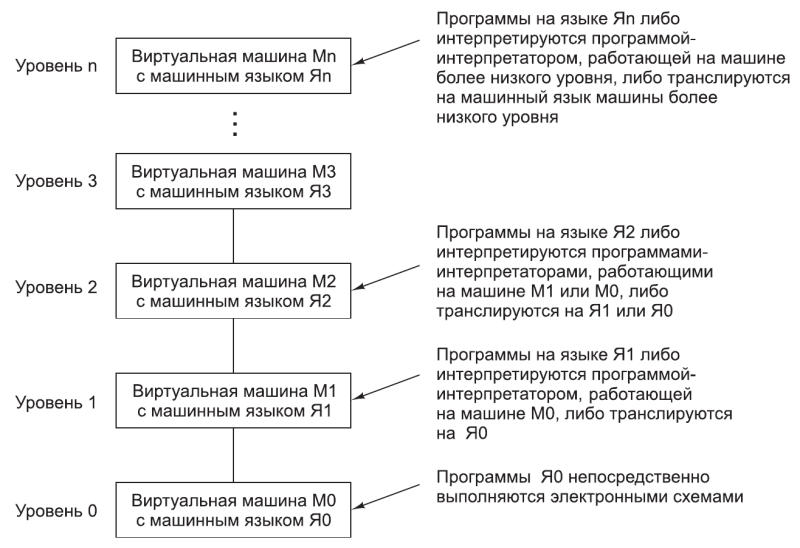
\includegraphics[width=1.0\textwidth]{img/definition-01.png}
  \caption{Понятие многоуровневости архитектуры по Э.\,Танненбауму}
  \label{definition-01}
\end{figure}

Он также приводит конкретную иеррархию уровней, построенную по этой схеме, которая приведена на рисунке~\ref{base-02}.

\begin{figure}[htbp]
  \centering
  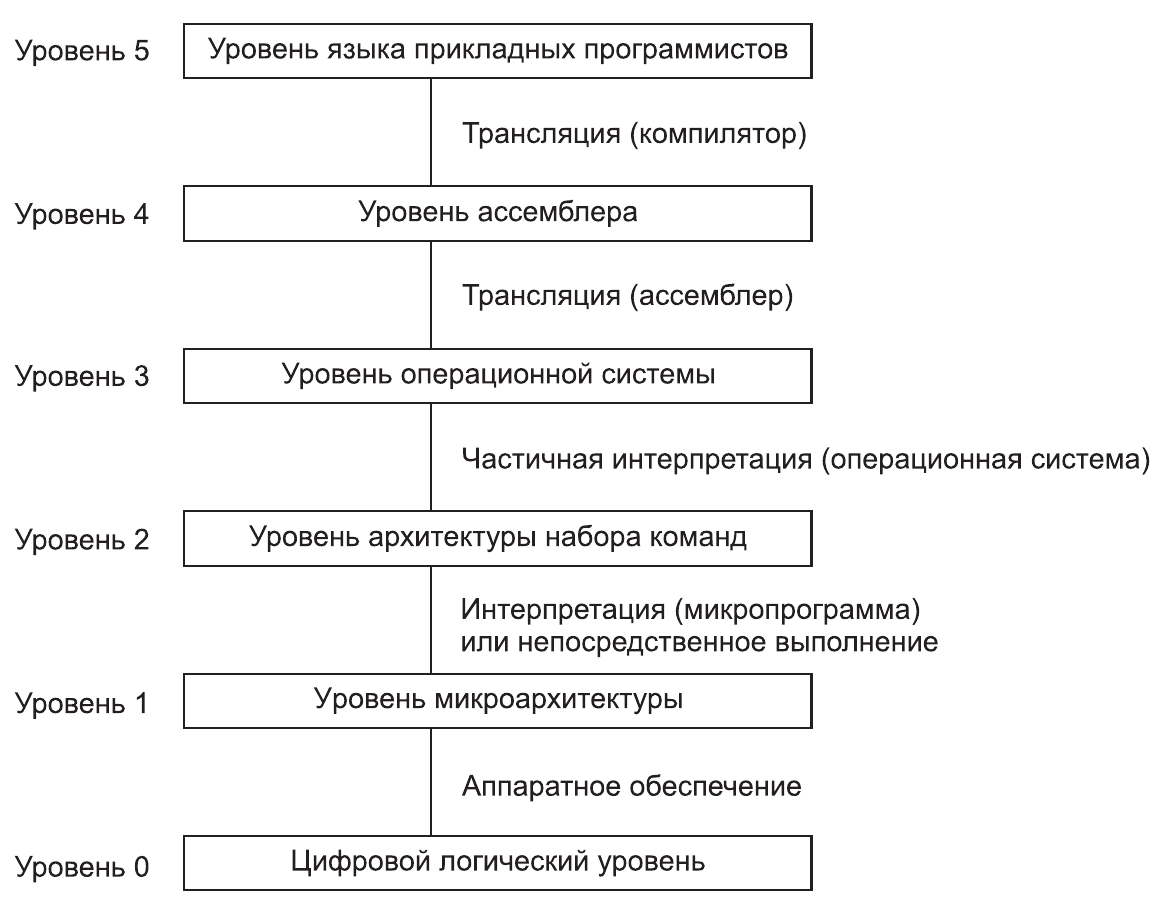
\includegraphics[width=1.0\textwidth]{img/base-02.png}
  \caption{Многоуровневая архитектура ВС по Э.\,Танненбауму}
  \label{base-02}
\end{figure}

Вместе с тем следует отметить, что можно предствить и большую детализацию уровней, что обуславливается спецификой использования каждого из них в современном процессе разработки программного обеспечения и широкого использования промежуточных виртуальных архитектур. Она будет выглядеть следующим образом:

\begin{itemize}
    \item Уровень предметно--ориентированных (специализированных) языков (Norma, ANTLR, GPSS, Prolog, Cmake...)
    \item Уровень универсальных языков прикладного программирования (Java, Kotlin, C\#, Python, Go, JS...)
    \item Уровень языков ориентированных на системное программирования (C, C++, Rust...)
    \item Уровень промежуточных языков (LLVM, MSIL, JavaVM...)
    \item Уровень ассемблера
    \item Уровень операционной системы
    \item Уровень архитектуры набора команд
    \item Уровень микроархитектуры
    \item Цифровой логическиий уровень
\end{itemize}

Весьма часто в профессиональной деятельности возникает необходимость ориентации в как в прикладных аспектах решаемой задачи так и в эффективном отображениии на используемую ВС. То есть в рассмотрении решаемой задачи с позиций нескольких архитектурных уровней восприятия. Это может быть связано со следующими факторами:

\begin{itemize}
    \item Многие классы задач требуют понимания и использования разнообразных по уровню компьютерных архитектур.
    \item Часто в компаниях перебрасывают программистов с одного проекта на другой. При этом изменяются характеристики языковых и инструментальных средств, определяющих специфику уровней архитектуры.
    \item Некоторые направления предметной области изменяются за счет автоматизации, отсутствия спроса и по другим причинам. Это ведет к необходимости переориентации на другие задачи, зачастую меняющие уровень используемой компьютерной архитектуры.
    \item Незнание методов и подходов других архитектурных уровней зачастую ведет к неэффективному решению поставленной задачи за счет неправильно выбора инструментов, которые соответствуют текущим знаниям разработчика, но не соответствуют архитектурному уровню решаемой задачи. При этом возможны:
    \begin{itemize}
        \item несоответствие вниз, когда незнание более низких уровней ведет к потере эффективности при работе программы на реальной ВС;
        \item несоответствие вверх, когда процесс разработки программного обеспечения становится менее эффективным, за счет неправильного выбора инструментов.
    \end{itemize}
\end{itemize}

Каждый архитектурный уровень не обязательно должен поддерживаться соответствующими инструментальными средствами. Зачастую один и тот же инструмент, ориентированный на конкретный архитектурный уровень, обеспечивает поддержку как вышележащих, так и нижележащих уровней. Подобными качествам обладает практически любой язык программирования. В качестве примера можно привести C++. Несмотря на то, что он в основном позиционируется как язык системного программирования, наличие таких абстракций как функции и классы позволяют создавать библиотеки, которые могут позиционироваться как поддержка вышестоящих уровней. В качестве примера покрытия различных уровней можно привести:

\begin{itemize}
    \item поддержка предметно--ориентированного или специализированного программирования с использованием библиотек SFML, SDL и других;
    \item поддержка универсального программирования на прикладном уровни, реализуемого с использованием стандартной библиотеки языка или библиотеки Boost;
    \item на уровне системного программирования непосредственно используются средства самого языка и ряда специализированных библиотек;
    \item поддержка уровня системы команд обеспечивается встроенным ассемблером.
\end{itemize}

% --- Отображение предметной области на многоуровневые архитектуры ---
% 2. Отображение предметной области на многоуровневые архитектуры

\chapter{Отображение предметной области на многоуровневые архитектуры}

Разработка больших программ – многоступенчатый процесс, в ходе которого осуществляются как ручные трансформации неформальных моделей решаемой задачи в формализованные представления, так и их последующая автоматическая трансформация с использованием различных систем программирования.

\begin{itemize}
    \item Предметная область
    \item Архитектура ВС
    \item Инструменты для разработки ПО
\end{itemize}

\begin{figure}[htbp]
    \centering
    
\includegraphics[width=0.8\textwidth]{img/reflection-02.png}
    \caption{Три кита, определяющие процесс разработки программ}
    \label{reflection-02}
\end{figure}

\section{Влияние особенностей архитектур вычислительных систем («железо», ОС, ЯП)}

\begin{itemize}
    \item время выполнения программы
    \item особенности программирования
    \item особенности оборудования
    \item …
\end{itemize}

Помимо увязки моделей предметной области с архитектурой ВС, встают проблемы, определяемые спецификой инструментов, используемых для создания программ.

Можно выделить технологическое направление, напрямую не связанное с предметной областью.

В его рамках формулируются требования:

\begin{itemize}
    \item к средствам, обеспечивающим написание программ,
    \item к средствам проектирования, определяющим переход от моделей предметной области к программам.
\end{itemize}

Огромную роль на разработку ПО оказывает необходимость соответствия заданным критериям качества.
Ряд критериев вытекает из особенностей предметной области. Другие обуславливаются архитектурой ВС и другими причинами.

\textbf{Вместе они характеризуют комплекс проблем, преодолеть который пытаются разработчики программного обеспечения.}

\section{Критерии качества программного обеспечения}

Применение информационных технологий немыслимо без создания программного обеспечения (ПО), разработка которого зачастую является сложным многоступенчатым процессом. Существуют альтернативные взгляды на этот процесс. Но в целом он связан с построением различных моделей, начиная от моделей предметной области и заканчивая моделями, воплощенными в законченном программном продукте. При этом осуществляются ручные трансформации неформального представления предметной области, определяющего понятия решаемой задачи, в ее формализованное представление. Полученные модели описываются в виде программ на языках программирования, после чего происходит их трансформация в машинные коды. Предметная область во многом определяет специфику разрабатываемых приложений, характеризуя состав и особенности используемых моделей, создание которых бывает весьма сложным и многогранным. Их окончательная структура может формироваться не только во время написания программы, но и в ходе ее выполнения за счет динамического связывания.

В немалой степени на процесс программирования влияют также особенности компьютеров, недооценка которых может привести к резкому снижению эффективности процесса обработки данных. Это обуславливается нюансами их внутренней организации, ориентацией на различные предметные области, и проявляется для программистов через компьютерную архитектуру, а также языки и системы программирования.

Наряду с необходимостью увязки моделей предметных областей и архитектур вычислительных систем, перед программистами встают проблемы, решение которых определяется спецификой инструментов, используемых для создания программ. Попытки решить их привели к выделению технологического направления, напрямую не связанного с предметной областью. В его рамках формулируются требования как к средствам кодирования, обеспечивающим написание программ, так и к средствам проектирования, определяющим переход от моделей предметной области к программам.

Между системами программирования и методами разработки ПО нет четкой грани. Существует их взаимное влияние друг на друга вне зависимости от используемых подходов и технических средств. Совместное использование заключается в том, что методы проектирования применяются для «ручного» перехода от исходных моделей к программам, а системы программирования обеспечивают непосредственное написание программ и их автоматический перевод в язык конкретного исполнителя. Например, объектно-ориентированная методология (ООМ) предлагает унифицированный процесс проектирования, инструментальная поддержка которого обеспечивает непосредственное построение каркасов программных приложений. Совместное использование методик проектирования и систем программирования осуществляется также при других методах разработки программного обеспечения.

В рамках технологии программирования проводятся исследования методов разработки, обеспечивающих создание продуктов, соответствующих заданным критериям качества. Ряд этих критериев вытекает из особенностей построения моделей предметной области. Другие обуславливаются сугубо внутренними причинами. Вместе они характеризуют комплекс проблем, преодолеть который пытаются разработчики систем программирования. Некоторые из критериев учитывают правила конструирования и технику написания программы. В частности, к ним относятся:

\begin{itemize}
    \item Корректность (правильность). Программа обеспечивает правильную обработку на правильных данных.
    \item Устойчивость. Программа «элегантно» завершает обработку ошибок.
    \item Расширяемость. Программа может легко адаптироваться к изменяющимся требованиям.
    \item Многократность использования. Программа может использоваться и в других системах, а не только в той, для которой было создана.
    \item Совместимость. Программа может легко использоваться с другим программным обеспечением.
    \item Эффективность. Обеспечивается эффективное использование времени, компьютерной памяти, дискового пространства и т.д.
    \item Переносимость. Разработанное программное обеспечение можно легко перенести на другие аппаратные и программные средства.
    \item Верификация. Простота проверки, легкость разработки тестов при обнаружении ошибок, легкость обнаружения мест, где программа потерпела неудачу, и т.д.
    \item Поддержка целостности. Программа защищает себя от неправильного обращения и неправильного употребления.
    \item Легкость использования. Не возникает проблем для пользователя в эксплуатации программы, а для будущих программистов в ее дальнейшем сопровождении и развитии.
\end{itemize}

Невозможно сопоставить важность указанных характеристик, так как все они, в той или иной степени, должны учитываться при разработке программного обеспечения. Вместе с тем следует отметить их относительную независимость, что позволяет сконцентрировать исследования на более тщательной проработке отдельных компонент перспективных систем программирования, отвечающих за конкретные критерии качества.

Не следует пренебрегать и организационными аспектами процесса разработки ПО, определяющими построение коллектива разработчиков, распределение ролей на выполнение различных видов работ. Это один из существенных факторов, во многом определяющих успешность создания требуемого программного продукта. Именно вокруг того, как организовать работу над программным проектом постоянно идут оживленные дискусси и ломаются копья. Однако в данном материале я не буду заострять внимание на этом важном с точки зрения реального проектирования вопросе, акцентировав основное внимание на технической, а не организационной стороне.

\subsection{Факторы, определяющие процесс разработки программного обеспечения}

Среди множества факторов, от которых зависит процесс разработки программного обеспечения, можно выделить:

\begin{itemize}
    \item классы решаемых, задач, определяющие смысловое содержание создаваемых программ;
    \item методологии, задающие особенности организационного и технического проведения основных этапов разработки программного обеспечения;
    \item методы и парадигмы программирования, обуславливающих стили кодирования и архитектуры виртуальных машин;
    \item аппаратные и системные программные средства, предоставляющие виртуальные и физические ресурсы для непосредственного использования ПО.
\end{itemize}


Разнообразие этих факторов определяет множество вариантов, связанных с организацией процесса разработки. Определим его основные составляющие.

Цель процесса разработки – создание программы, обеспечивающей решение поставленной задачи некоторым исполнителем и удовлетворяющей при этом требуемым критериям качества. Решаемая задача описывается совокупностью формальных и эмпирических (неформальных) моделей, определяющих как протекающие в программе процессы, так и используемые при этом данные.

Модель задачи – совокупность специализированных моделей, описывающих различные аспекты решаемой задачи, отражаемые в разрабатываемой программе.

Специализированная модель – модель, предназначенная для описания определенных параметров рассматриваемого явления. Используется для акцентирования внимания на частных характеристиках.

Разрабатываемая программа должна обеспечивать выполнение функций, необходимых для решения задачи, в соответствующем исполнителе (вычислительной системе), специфика которого отражается в его модели.

Модель исполнителя – совокупность специализированных моделей, описывающих организацию и поведение вычислительной системы, осуществляющей выполнение программы.

Создаваемая программа является отображением модели решаемой задачи на модель исполнителя. Общая схема этого процесса разработки представлена на рисунке~\ref{fig01-01}. Трудоемкость программирования, с одной стороны, определяется количеством специализированных моделей, описывающих задачу, их размером, семантическим отличием от специализированных моделей исполнителя. С другой стороны она зависит от характеристик модели исполнителя, задающей требования к уровню абстракции разрабатываемой программы и ее приближенностью к архитектуре реального вычислителя.

\begin{figure}[htbp]
    \centering
    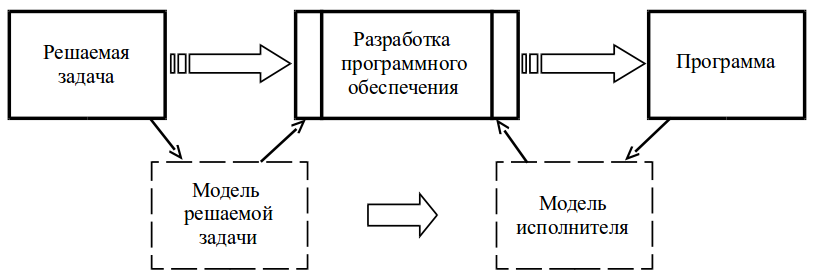
\includegraphics[width=0.9\textwidth]{img/fig01-01.png}
    \caption[Процесс разработки ПО]{Процесс разработки программного обеспечения как отображение модели задачи на модель исполнителя}
    \label{fig01-01}
\end{figure}

Сложность модели задачи может потребовать ее поэтапного преобразования в модель исполнителя, что схематически представлено на рисунке~\ref{fig01-02}. Необходимость в подобных преобразованиях обуславливается наличием семантического разрыва между моделями задач и исполнителей. Он проявляется в том, что объекты и операции, которыми разработчик манипулирует при описании задачи, не совпадают с объектами и операциями, используемыми при построении программы. Преодоление семантического разрыва осуществляется использованием методических и технических приемов, повышающих, к тому же, эффективность процесса разработки ПО.

\begin{figure}[htbp]
    \centering
    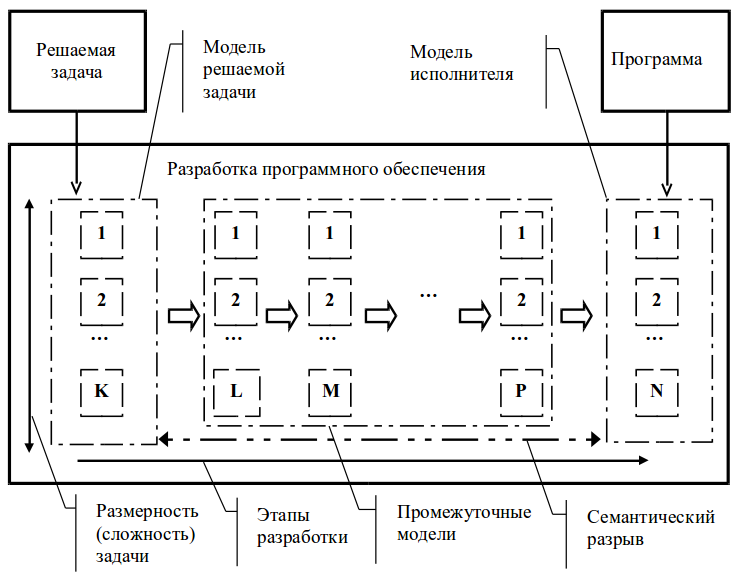
\includegraphics[width=0.9\textwidth]{img/fig01-02.png}
    \caption[Сложность преобразования моделей]{Влияние сложности задачи на процесс преобразования исходных моделей в модели исполнителя}
    \label{fig01-02}
\end{figure}

Разбиение моделей по различным этапам позволяет оценить объем работ на каждом из них. Помимо этого можно получить и временные характеристики как для каждого этапа, так и для всего процесса разработки ПО в целом. Общий объем работ определяется суммарным объемом, связанным с построением всех специализированных моделей. Условно это представлено на рисунке~\ref{fdiag01}.

\begin{figure}[htbp]
    \centering
    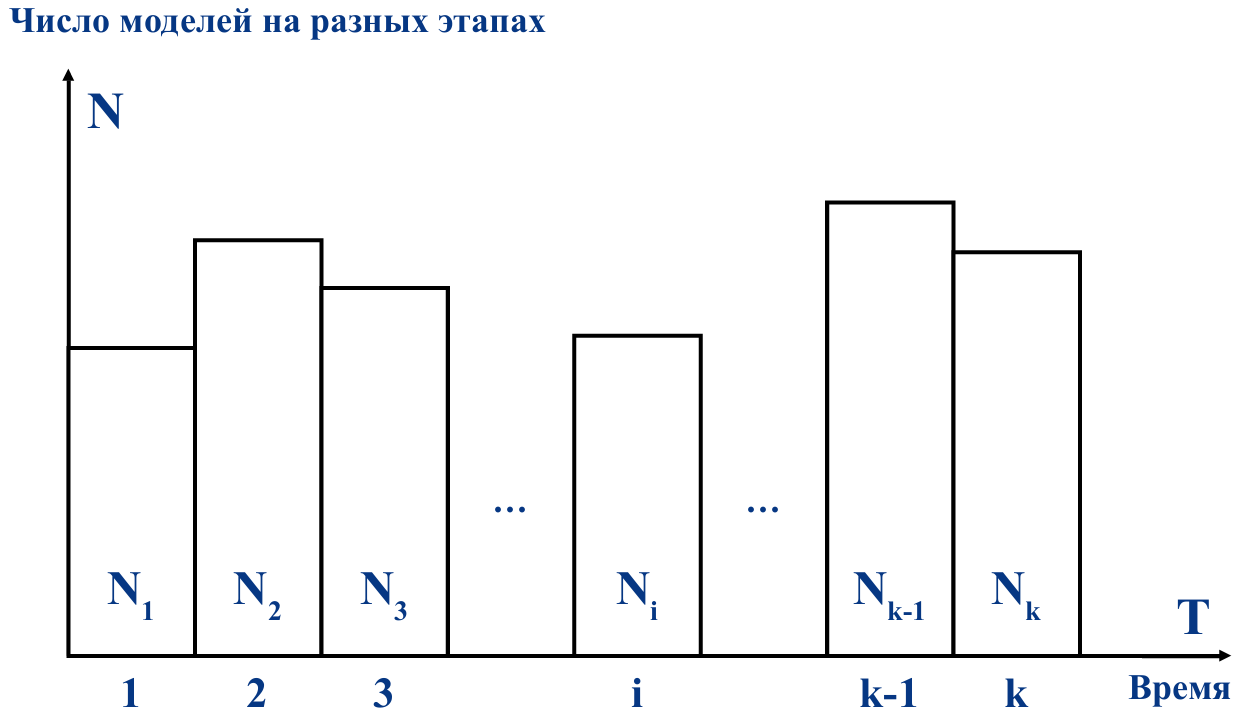
\includegraphics[width=0.9\textwidth]{img/fdiag01.png}
    \caption{Отображение объема работ и времени их выполнения в ходе разработки ПО}
    \label{fdiag01}
\end{figure}

\subsection{Методические приемы}

\textbf{Методические приемы} ориентированы на формализацию представления моделей и методов перехода между ними. Они позволяют ускорить процесс разработки следующими способами:

\begin{itemize}
    \item формализацией предметных областей;
    \item созданием методик разработки программного обеспечения.
\end{itemize}

\subsubsection*{Формализация предметной области}

Формализация предметной области заключается в построении ее модели и разработке методов преобразования модели предметной области в модель исполнителя. Модель предметной области объединяет совокупность специализированных моделей предназначенных для описания определенного класса решаемых задач, что обеспечивают ограничения на формируемое решение сверху. Дальнейший переход к модели исполнителя обычно осуществляется по выработанным методам или алгоритмам (рисунок~\ref{fig01-03a}).

\begin{figure}[htbp]
    \centering
    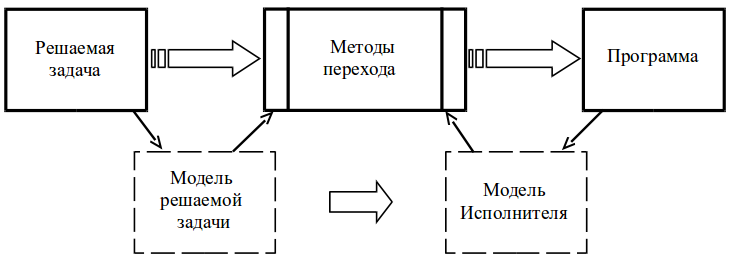
\includegraphics[width=0.9\textwidth]{img/fig01-03a.png}
    \caption{Формализация предметной области за счет разработки методов перехода от модели решаемой задачи к программе}
    \label{fig01-03a}
\end{figure}

Подобный подход широко используется при разработке программ в разных предметных областях. В качестве примеров, можно привести:

Построение синтаксических и лексических анализаторов. Модель предметной области, то есть язык программирования, описывается с использованием формальных грамматик, определяющих принципы порождения правильных цепочек языка. Наличие эквивалентности между различными грамматиками и автоматами позволяет перейти к распознавателям цепочек путем использования наработанных методов их программной реализации.

Разработка программных систем на основе теории автоматов, например, автоматное программирование. Последующая программная реализация автоматов является хорошо отработанным формальным приемом с применением различных технологий.

Основной эффект достигается за счет того, что при проработке и/или формализации методов используются уже полученные знания, что позволяет ускорить построение требуемых моделей. Это, в свою очередь, сокращает общий объем выполняемых работ и время выполнения процесса разработки (рисунок~\ref{fdiag02}).

\begin{figure}[htbp]
    \centering
    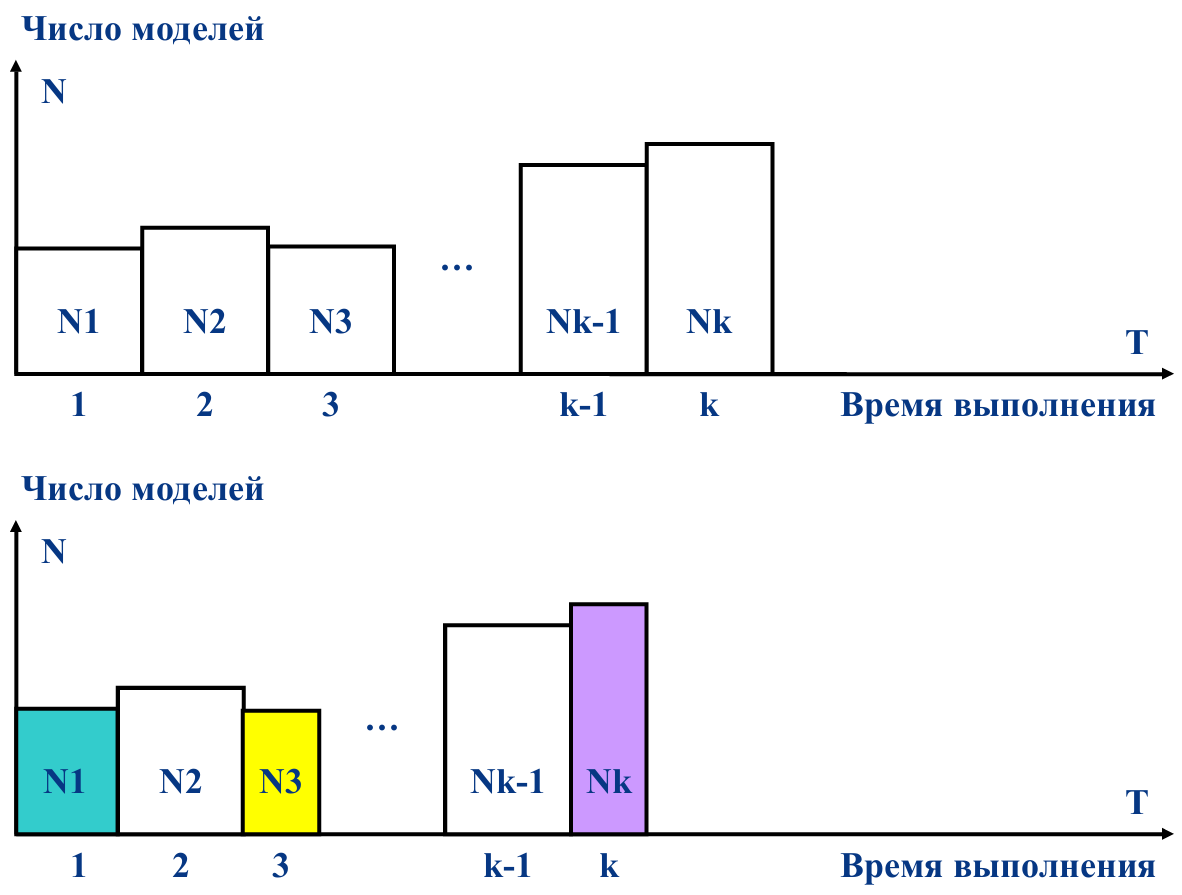
\includegraphics[width=0.8\textwidth]{img/fdiag02.png}
    \caption{Сокращение премени выполнения работ за счет формализации моделей}
    \label{fdiag02}
\end{figure}

Разработка алгоритмов преобразования одних моделей в другие позволяет автоматизировать процесс и обеспечить представление исходной задачи в виде формализованных данных или программы на специализированном (про\-блем\-но--ориентированном или предметно--ориентированном) языке программирования. Фактически это означает слияние моделей задачи и исполнителя (рисунок~\ref{fig01-03b}).

\begin{figure}[htbp]
    \centering
    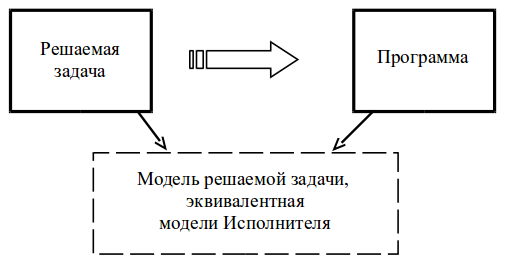
\includegraphics[width=0.7\textwidth]{img/fig01-03b.png}
    \caption{Разработка системы программирования, соответствующей предметной области ведет к непосредственному описанию решаемой задаче и слиянию моделей}
    \label{fig01-03b}
\end{figure}

По такой схеме разрабатываются различные предметно-ориентированные и специализированные языки, а также соответствующи системы программирования. К ним, в частности, можно отнести:

многие языки имитационного моделирования, обеспечивающие непосредсвенное описание моделей (можно отметить такие языки как GPSS, AnyLogic и другие);

системы автоматизированной генерации лексических и синтаксических анализаторов языков программирования по описанию синтаксиса на соответствующих метаязыках (начиная от таких первопроходцев как lex и yacc);

языки международного стандарта IEC 61131-3, ориентированные на разработку ПО логических контроллеров.

В этом случае временные характеристики процесса разработки можно представит в виде исходных моделей предметной области и моделей виртуального исполнителя, программируемого на специализированном или проблемно-ориентированном языке (рисунок~\ref{fdiag03}).

\begin{figure}[htbp]
    \centering
    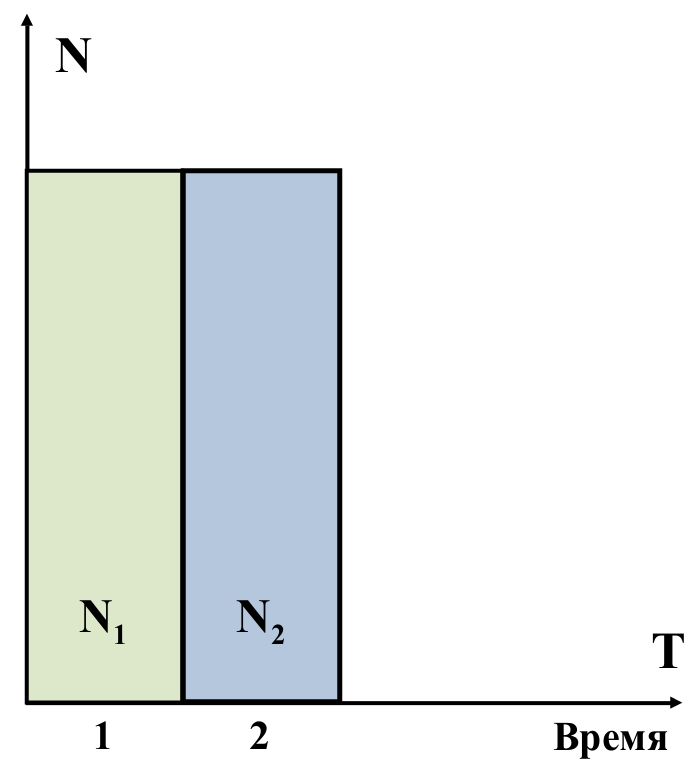
\includegraphics[width=0.4\textwidth]{img/fdiag03.png}
    \caption{Использование специализированного языка для описания моделей предметной области (идеализированный вариант)}
    \label{fdiag03}
\end{figure}

Следует отметить, что помимо языков и специальных сред разработки проблемная ориентация, а следовательно и определенная формализация предметной области, осуществляется за счет использования библиотек в рамках различных универсальных языков программирования. В частности следует отметить разнообразные библиотеки, повышающие эффективность разработки компьютерных игр.

Достоинства подхода, опирающегося на формализацию предметной области, проявляются в следующем:

\begin{itemize}
    \item достижение более высокой скорости разработки программ (к программированию можно приступать уже во время анализа решаемой задачи);
    \item разработкой могут заниматься специалисты-предметники, не являющиеся профессионалами в программировании;
    \item программирование может протекать непосредственно в терминах предметной области, что еще больше повышает эффективность процесса разработки (программирование без программирования).
\end{itemize}


К недостаткам подхода следует отнести:

\begin{itemize}
    \item отсутствие гибкости (предметная ориентация моделей не позволяет непосредственно использовать накопленные методы и инструменты в других областях);
    \item ориентацию на достаточно узкую категорию задач;
    \item необходимость разработки и использования специализированных инструментальных средств.
\end{itemize}

Прием эффективен при решении достаточно простых задач узкого класса, так как увеличение размерности резко повышает количество применяемых специализированных моделей, пригодных для использования в разнообразных предметных областях. Это ведет к увеличению сложности методов формализации и уменьшению эффективности комплексного использования специализированных моделей.

С формализацией предметной области достаточно тесно связан предметно-ориентированный подход к проектированию (Domain--driven design, DDD). Эта связь проявляется в более внимательном изучении контекста прикладной области, выделении в ней различных факторов, для которых можно обеспечить построение более строгих моделей, поддающихся дальнейшей формализации. Наряду с этим в ходе такого проектирования часто формируется язык предметной области, который может быть реализован либо с использованием средств существующих языков программирования, либо путем создания соответствующего специализированного или предметно-ориентированного языка.

В заметке «Формализация предметной области на примере вычисления 100!» представлен простой пример, демонстрирующий специфику данного методического приема.

\subsubsection*{Создание методик разработки программного обеспечения}

Методики разработки программного обеспечения ориентированы на формализацию взаимосвязей между моделями конкретных исполнителей и моделями, используемыми на предшествующих этапах разработки (например, при анализе и проектировании). Место методик (состоящих из набора методов преобразования между различными группами моделей) в процессе разработки ПО представлено на рисунке~\ref{fig01-04}.

\begin{figure}[htbp]
    \centering
    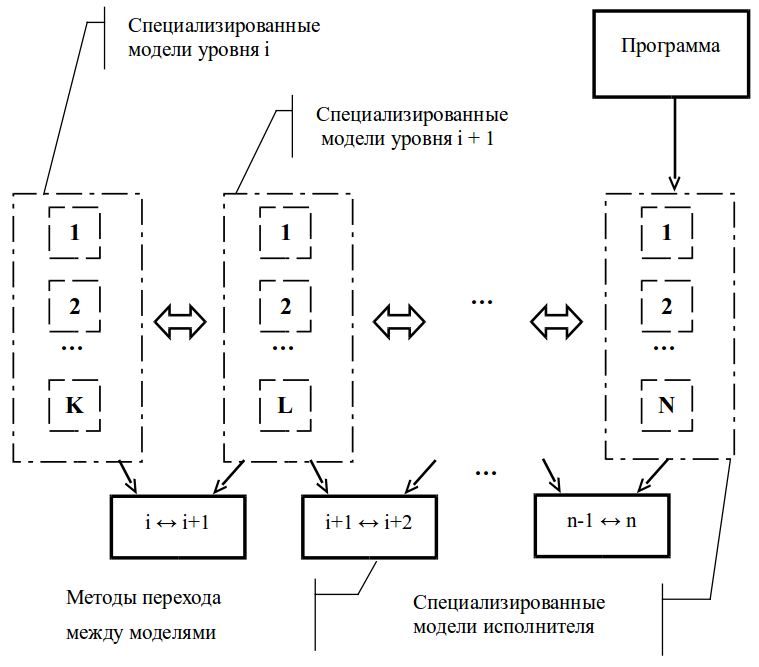
\includegraphics[width=0.9\textwidth]{img/fig01-04.png}
    \caption{Использование методик разработки для поэтапного преобразования моделей}
    \label{fig01-04}
\end{figure}

Изначальная ориентация Исполнителя на универсальность вычислений обычно предполагает применение методик для широкого класса задач, не связывая их непосредственно с предметными областями. Они поддерживают взаимодействие моделей, используемых в разработке, определяя процесс преобразования как от модели задачи к модели исполнителя, так и в обратном направлении.

Несмотря на обеспечение прямого и обратного проектирования, основное достоинство методик проявляется в поддержке нисходящей разработки, что во многом обуславливается большей наглядностью переходов от универсальных высокоуровневых моделей предметных областей к моделям, описывающим соответствующих исполнителей. В подобной ситуации знание задачи повышает эффективность разработки. Поэтому, создание программного обеспечения обычно начинается с привязки модели предметной области к моделям анализа и проектирования, предлагаемым используемой методикой (рисунок~\ref{fig01-05}).

\begin{figure}[htbp]
    \centering
    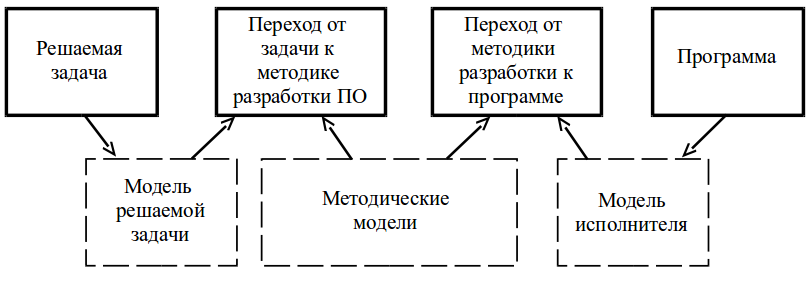
\includegraphics[width=0.9\textwidth]{img/fig01-05.png}
    \caption{Использование методик разработки в виде методических моделей}
    \label{fig01-05}
\end{figure}

Применение методических моделй не влияет непосредственно на скорость разработки специализированных моделей. Однако это позволяет сократить время переходов между различными взаимозависимыми моделями, что в конце концов можно трактовать как сокращение времени перехода между различными этапами процесса разработки. Условно это сокращение показано на рисунке~\ref{fdiag04}.

\begin{figure}[htbp]
    \centering
    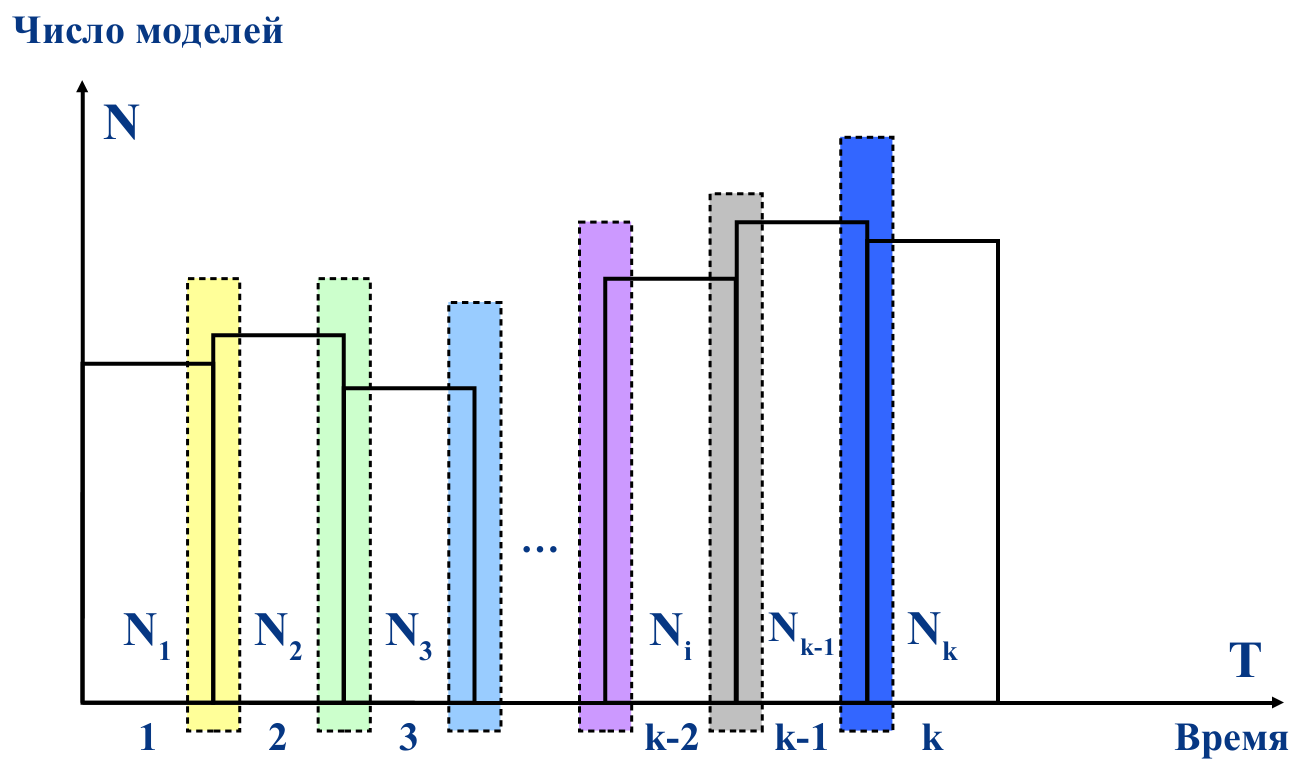
\includegraphics[width=0.9\textwidth]{img/fdiag04.png}
    \caption{Сокращение времени разработки ПО за счет использования методических моделей}
    \label{fdiag04}
\end{figure}

К достоинствам методик разработки ПО следует отнести:

\begin{itemize}
    \item универсальность, что позволяет ориентироваться на разработку задач широкого класса;
    \item поддержку нисходящего и восходящего проектирования;
    \item поддержку прямого и обратного проектирования;
    \item возможность использовать инструментальные средства.
\end{itemize}
К недостатку отдельных методик относится привязка процесса разработки к определенным методам и исполнителям.

В настоящее время существуют различные методики. Они являются составной и неотъемлемой частью методологий разработки программного обеспечения, которые, наряду с процессами создания программ, дополнительно регламентируют организационную деятельность, анализ, тестирование и сопровождение, что в целом определяет организацию жизненного цикла программы на основе единого концептуального подхода. Примерами подобных методик могут служить:

\begin{itemize}
    \item объектно-ориентированный подход, используемый в составе объектно-ориентированной методологии;
    \item методы структурного анализа и проектирования (structured analysis and design technique, SADT), часто применяемые при разработке информационных систем;
    \item методы быстрой разработки приложений (rapid application development, RAD), ориентированные на ускоренное построение программ от моделей, определяющих взаимодействие системы с пользователем.
\end{itemize}

Методики широко используются при разработке больших программных систем, так как повышают эффективность проектирования за счет предоставления достаточно простых и ясных подходов, выработанных на основе эмпирического опыта и теоретических исследований. Их использование, в сочетании с инструментальной поддержкой, обеспечивает сокращение семантического разрыва между моделями задач и исполнителем.

\subsection{Технические приемы}

Технические приемы ориентированы на использование инструментальных средств, поддерживающих различные аспекты процесса разработки ПО. Можно выделить:

\begin{itemize}
    \item средства поддержки методических приемов;
    \item вспомогательные средства;
    \item системы программирования.
\end{itemize}

\subsection*{Поддержка методических приемов}

Инструментальные средства, обеспечивающие поддержку методических приемов, предназначены для компьютерного представления и анализа разрабатываемых моделей, преобразования построенных моделей в другие модели, автоматизации процесса построения требуемой документации, а также ведения организационной деятельности в ходе разработки ПО. Повышая эффективность процесса разработки, средства поддержки методических приемов, в то же время, не определяют сам процесс создания программы. Их использование предполагает дальнейшую доводку программ с применением инструментов, имеющих более тесную связь с архитектурами вычислительных систем.

Примерами ранних средств подобного рода могут служить системы поддержки спецификаций. Во многих из них использовались графические языки, которые в основном играли роль вспомогательного документа. Для написания программы необходимо было вручную осуществлять перевод этих диаграмм в код. Положение изменилось с внедрением CASE-средств. Разработанные инструменты сгладили семантический разрыв между рядом моделей предметной области и кодом, обеспечив непосредственное преобразование, как в прямом, так и в обратном направлении. К средствам поддержки методов структурного анализа и проектирования можно отнести, например, различные системы, обеспечивающие инструментальную поддержку UML, и, следовательно, объектно-ориентированную и другие методологии.

\subsubsection{Вспомогательные средства}

Вспомогательные средства предназначены для повышения эффективности процессов, не связанных с непосредственной разработкой структуры программы, но, в то же время, сильно влияющих на качество и время разработки. К ним следует отнести:

\begin{itemize}
    \item средства отладки программ;
    \item системы тестирования;
    \item средства профилирования и другие.
\end{itemize}

Их специфика заключается в работе с уже готовыми программами, что позволяет считать их влияние на процесс разработки программ косвенным образом.

Отладка используется для локализации и устранения ошибок в разрабатываемых программах. Существуют различные подходы к решению этой задачи. В частности проводятся следующие мероприятия:

\begin{itemize}
    \item анализируются текущие значения различных переменных;
    \item определяются траектории выполнения программы.
\end{itemize}


Эти задачи можно решать путем вставки к исходные тексты программ специальных вспомогательных операторов. Однако вместо этого часто используются специальные отладчики, которые повышают эффективность процесса отладки за счет дополнительных сервисных функций. Отладчики могут использоваться независимо от других инструментальных средств. Примером такого подхода является отладчик gdb. Однако зачастую отладчики непосредственно встраиваются в интегрированные среды разработки программ, что обеспечивает большую наглядность и оперативное исправление возникающих ошибок. К системам, ориентированным на такой подход можно отнести MS Visual Studio. Помимо этого, для повышения эффективности использования автономных отладчиков применяются дополнительные обертки в виде графических интерфейсов (например программа Data Display Debugger (ddd) формирует графический интерфейс вокруг отладчика gdb). Такие обертки могут также встраиваться и в интегрированные среды разработки, позволяя использовать один и тот же отладчик как автономно, так и внутри себя. В качестве примера такой среды можно выделить Qt Creator.

Тестирование заключается в проверке соответствия между реальным и ожидаемым поведением программы. Осуществляется на наборе тестов, подобранном определенным образом. Существуют разнообразные методы тестирования, которые обуславливаются особенностями процесса разработки программ на различных этапах. Это, в свою очередь, ведет к применению широкого набора разнообразных инструментальных средств, повышающих эффективность процесса разработки. Помимо этого тестирование может определять организацию процесса программирования, если используются методы разработки через тестирование (Test Driven Development — TDD).

Профилирование направлено на сбор и анализ характеристик, определяющих особенности функционирования программы. К ним относятся: время выполнения отдельных фрагментов кода (подпрограмм, функций, потоков, процессов), количество истинных и ложных переходов в различных условных операторах и операторах цикла, количество кэш промахов и т. д. Инструмент, предназначенный для получения этих характеристик, называется профилировщиком. Полученные данные используются для оптимизации программы повышающей эффективность ее функционирования, которая обычно связана с улучшением таких критериев качества как уменьшение времени выполнения программы, уменьшение объема занимаемой памяти и рядом других характеристик.

\subsubsection{Системы программирования}

Системы программирования – это инструментальные средства, поддерживающие разработку программ для заданного виртуального исполнителя и их последующее автоматическое преобразование в программы реального исполнителя.

Использование систем программирования позволяет решать задачу повышения эффективности процесса разработки ПО за счет сокрытия исполнителей более низкого уровня, являющихся реальными вычислительными системами (рисунок~\ref{fdiag05}). Такой подход широко используется на практике и позволяет писать программы для высокоуровневого исполнителя (определяемого часто как архитектура виртуальной машины).

\begin{figure}[htbp]
    \centering
    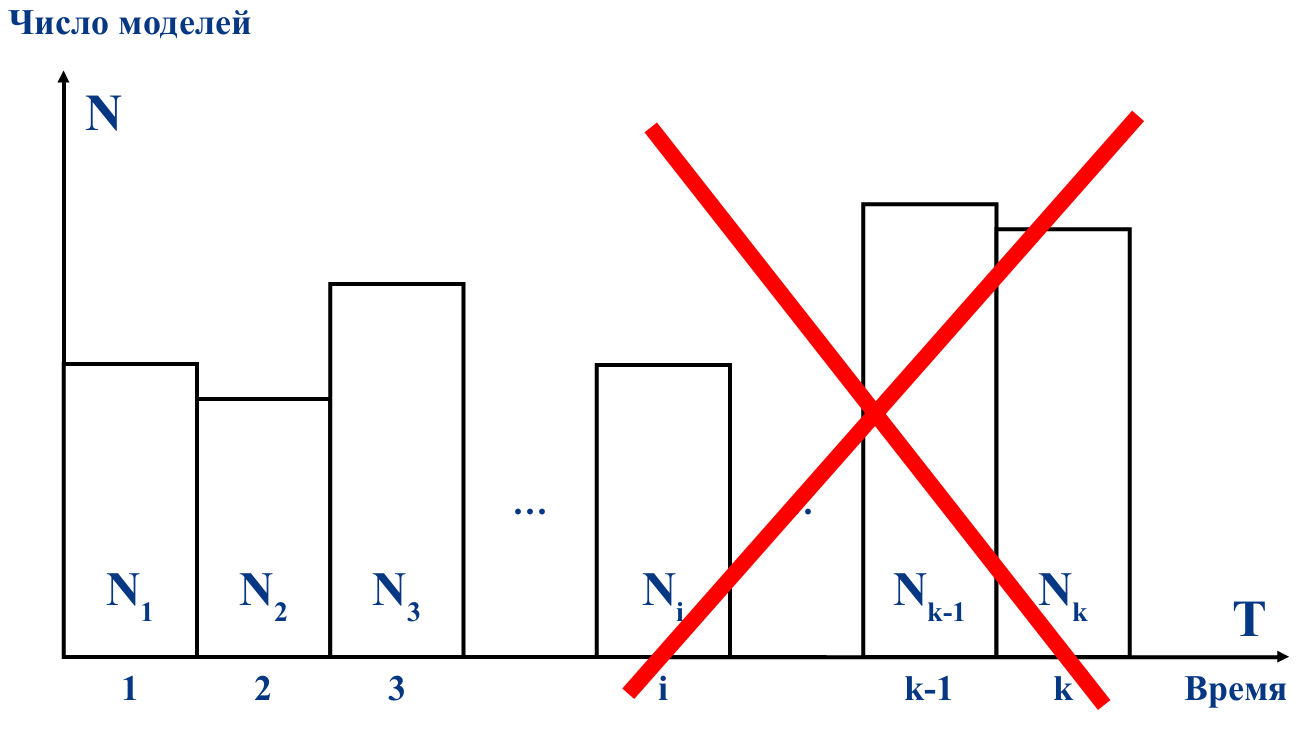
\includegraphics[width=0.9\textwidth]{img/fdiag05.png}
    \caption{Системы программирования «убирают» часть моделей из процесса разработки}
    \label{fdiag05}
\end{figure}


Выполнение полученных программ может осуществляться:

\begin{enumerate}
    \item Использованием непосредственной интерпретации, полностью скрывающей процесс реального выполнения, который может оказаться намного сложнее. Схема, иллюстрирующая подход, представлена на рисунке~\ref{fig01-06}.
\begin{figure}[htbp]
    \centering
    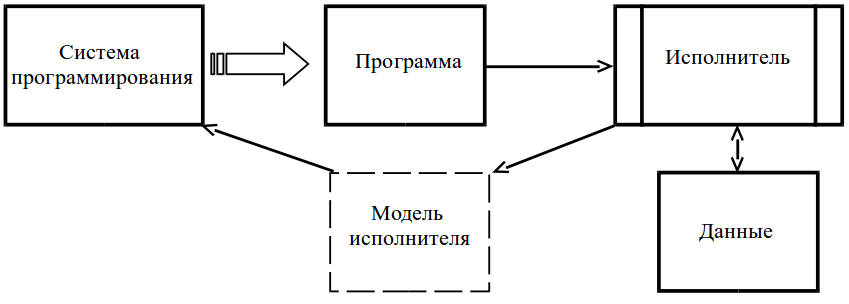
\includegraphics[width=0.9\textwidth]{img/fig01-06.png}
    \caption{Непосредственное использование исполнителем программы, написанной с применением системы программирования}
    \label{fig01-06}
\end{figure}
    \item Автоматическим и поэтапным преобразованием программы, написанной для виртуальной машины, в программу конечного исполнителя, обеспечивающего ее интерпретацию, что позволяет разрабатывать программы для систем, не допускающих непосредственное выполнение. Подобный прием применяется, например, в системах компиляции. Возможен вариант, когда преобразование программы является многоступенчатым, что может оказаться целесообразным при использовании нескольких промежуточных моделей исполнителей. Схема преобразований приведена на рисунке~\ref{fig01-07}. Проводимые промежуточные преобразования могут быть скрыты от программиста. Однако дополнительные знания о конечном исполнителе позволяют повысить эффективность процессов отладки и выполнения программы.
\end{enumerate}

\begin{figure}[htbp]
    \centering
    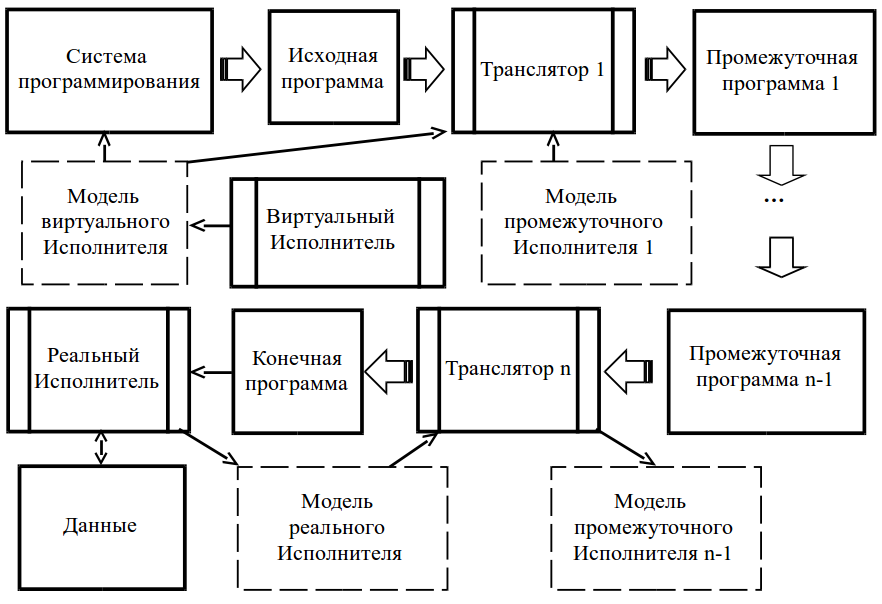
\includegraphics[width=0.9\textwidth]{img/fig01-07.png}
    \caption{Многоэтапное преобразование модели исполнителя, поддерживаемого системой программирования, в модель исполнителя, реально осуществляющего вычисления}
    \label{fig01-07}
\end{figure}

Каждый из представленных подходов может использовать одно и то же исходное представление программы. Их отличие проявляется на уровне дополнительных сервисов и знаний о моделях, применяемых в цепочке преобразований от исходного исполнителя до интерпретатора. В целом процесс работы конечного исполнителя не является определяющим для процесса разработки исходной программы.

Исполнители могут отличаться и по степени приближения их моделей к моделям решаемых задач или более высокоуровневым методологическим моделям. Использование в их архитектуре моделей решаемых задач ведет к разработке специализированных и проблемно-ориентированных систем программирования. Ориентация на общие модели проектирования обуславливает создание высокоуровневых универсальных средств. При ориентации на архитектуры реальных вычислительных систем можно разрабатывать более производительные программы. Однако процесс разработки усложняется за счет дополнительной детализации.


subsection{Связь между различными моделями процесса разработки и рассмотренной схемой}

В принципе представленный в заметке модельный взгляд отличается от существующих моделей жизненного цикла процесса разработки ПО только акцентом на другие параметры. Если рассматривать существующие подходы и классификации, то в них основное внимание уделяется этапам, а не их содержанию (речь идет о схемах, а не их детализации). В частности, в представленной на рисунке~\ref{fdiag06} водопадной модели четко выделены основные этапы процесса разработки, с каждым из которых связан свой комплекс работ и распределение ролей.

\begin{figure}[htbp]
    \centering
    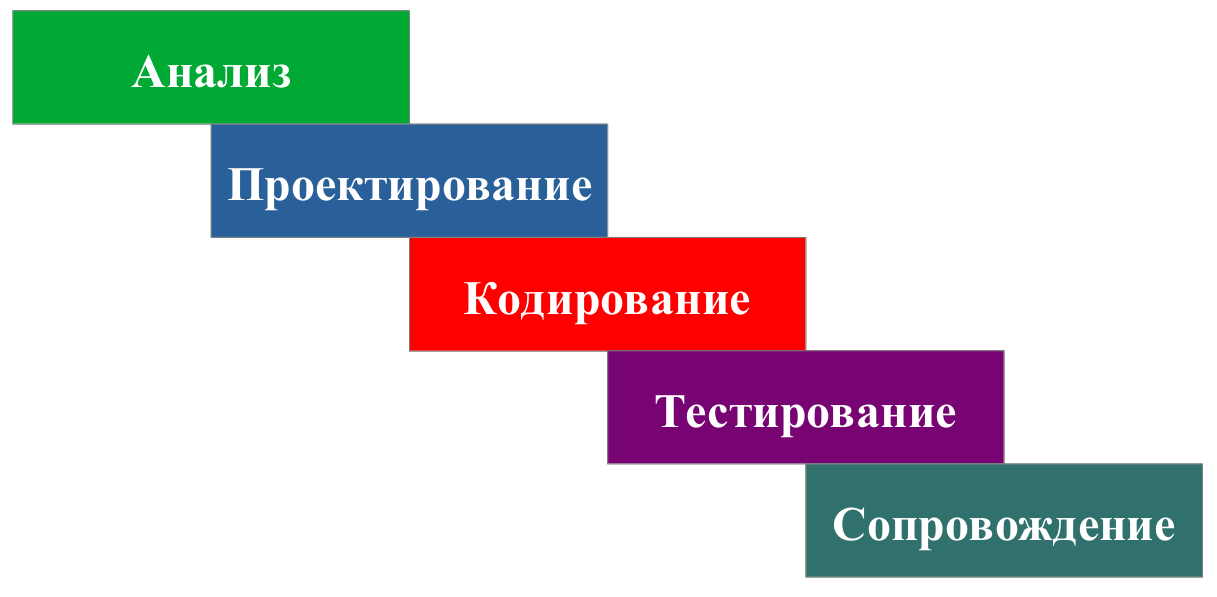
\includegraphics[width=0.9\textwidth]{img/fdiag06.png}
    \caption{Водопадная (каскадная) модель разработки ПО}
    \label{fdiag06}
\end{figure}

Ничто не мешает осуществить поэтапное разпределение и для специализированных моделей (рисунок~\ref{fdiag07}). Однако следует заметить, что и при этом основной упор в дальнейшей детализации будет направлен на характеристики моделей, а распределение работ между исполнителями будет связано не только с их разделением по этапам, но и с назначением им специализированных моделей внутри каждого из этапов.

\begin{figure}[htbp]
    \centering
    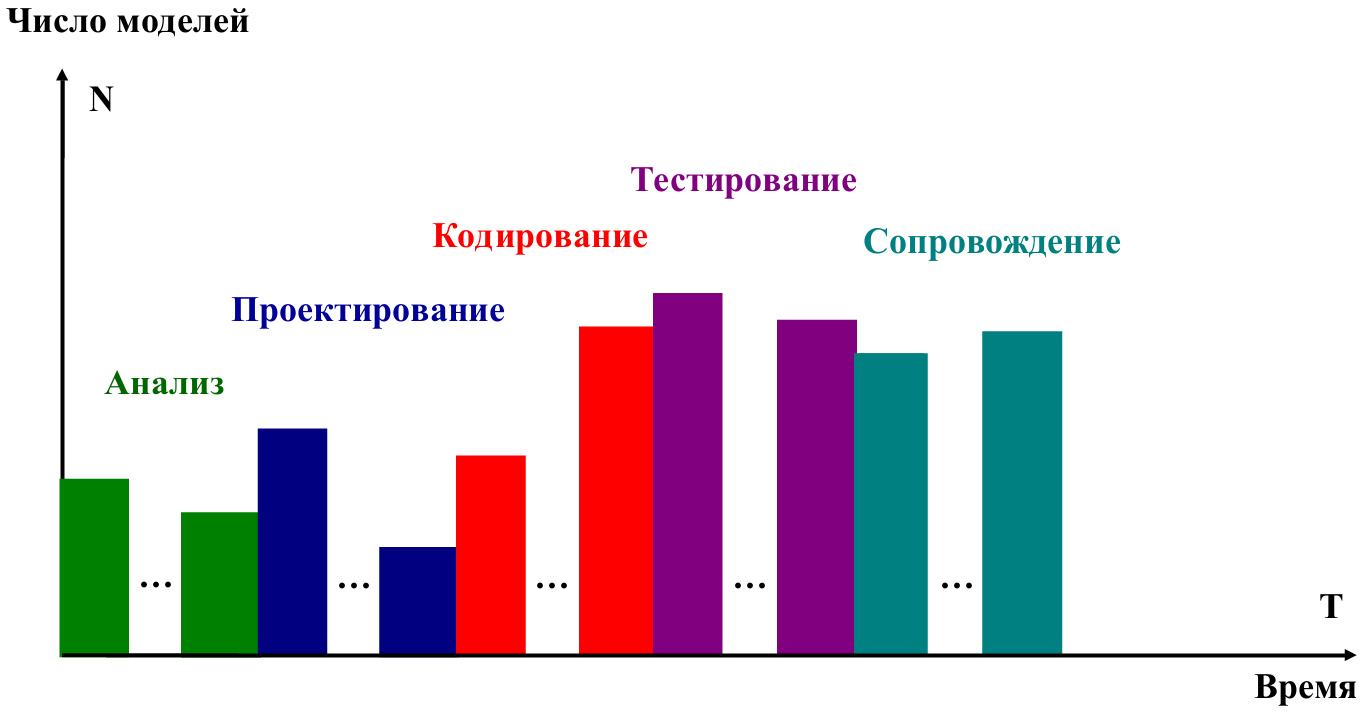
\includegraphics[width=1.0\textwidth]{img/fdiag07.png}
    \caption{Связь с водопадной моделью разработки ПО}
    \label{fdiag07}
\end{figure}

Аналогичным образом можно интерпретировать и итерационную (возвратную, спиральную) модель (рисунок~\ref{fdiag08}). Каждая очередная итерация заключается в повторении этапов разработки на каждом из которых выполняется расширение функциональности программного продукта.

\begin{figure}[htbp]
    \centering
    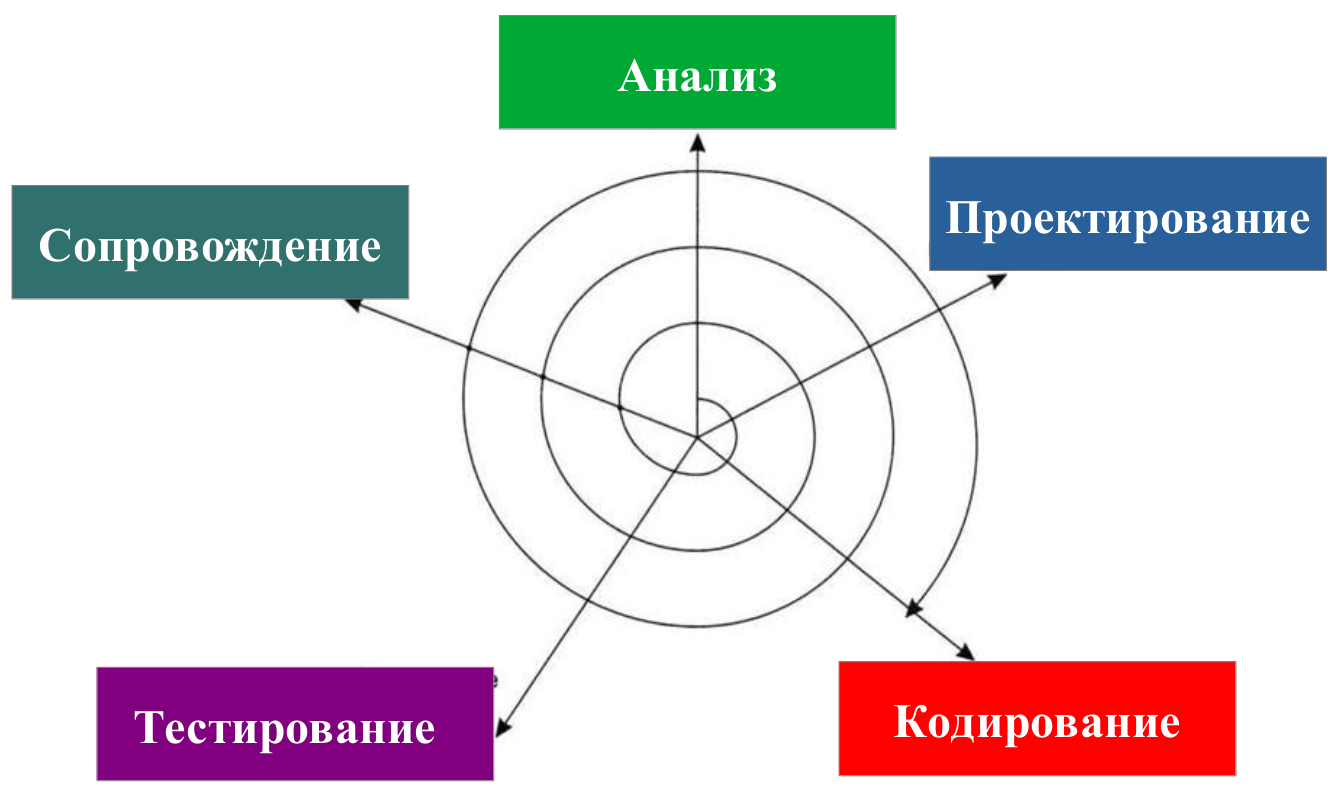
\includegraphics[width=1.0\textwidth]{img/fdiag08.png}
    \caption{Итерационная (возвратная) модель разработки ПО}
    \label{fdiag08}
\end{figure}

Это расширение можно интерпретировать как разработка только части моделей, распределенных по каждому из этапов (рисунок~\ref{fdiag09}). Помимо этого в модельной интерпретации можно также фиксировать зависимости между моделями отдельно для каждого витка итерации, стремясь при этом к тому, чтобы зависимости между моделями разных итераций были как можно меньше. Это ведет к тому, что планирование итераций на уровне специализированных моделей может дополнительно включать учет зависимостей между ними.

\begin{figure}[htbp]
    \centering
    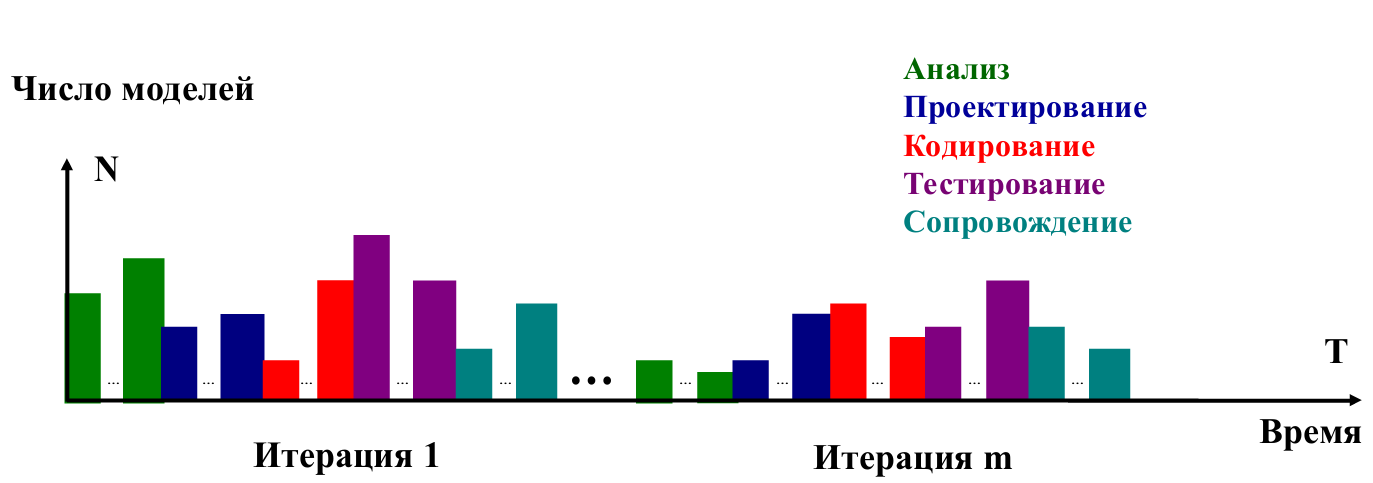
\includegraphics[width=0.9\textwidth]{img/fdiag09.png}
    \caption{Связь с итерационной моделью разработки ПО}
    \label{fdiag09}
\end{figure}

В целом следует отметить, что аналогичным образом можно взгляд модельный взгляд можно накладывать на различные модификации двух основны (рассмотренных выше) процессов разработки. Помимо этого в целом процесс разработки можно интерпретировать и независимо от этапов, акцентируя при этом внимание на определении специализированных моделей и установлении зависимостей между ними. На основании этого можно применять для процесса разработки ПО более гибкое планирование ресурсов и разработчиков.

\subsection{Выводы}

Рассмотрены основные понятия, связанные с процессом разработки программного обеспечения. Разработка программ непосредственно связана с использованием моделей, обеспечивающих описание решаемой задачи, применяемого исполнителя, промежуточных преобразований модели решаемой задачи в модель исполнителя. При этом между моделями решаемой задачи и моделями исполнителя существует семантический разрыв, преодоление которого осуществляется с использованием методологических и технических приемов, разнообразие которых определяется множеством различных факторов. Множество специализированных моделей может формироваться в зависимости от различных факторов. Повышение эффективности процесса разработки ПО во многом обеспечивается использованием соответствующих инструментальных средств.

\subsection{Вопросы}

\begin{enumerate}
    \item Опишите известную Вам предметную область. Какие модели необходимо задать для ее описания перед переходом к разработке программного продукта.
    \item Приведите характеристики компьютерных архитектур, используемых для выполнения программного обеспечения в известной Вам предметной области.
    \item Как проявляется семантический разрыв при разработке программного обеспечения? Какие существуют подходы для его сокращения?
    \item Приведите примеры известных Вам предметных областей, в которых применяютс методы формализаци.
    \item Какие из известных Вам методов формализации реализованы в виде систем или языков программирования?
    \item Приведите примеры предметно-ориентированных или специализированных языков, ориентированных на какую-либо предметную область. Как в этих языках отражается формализация предметной области?
    \item Приведите примеры библиотек, ориентированных на разработку компьютерных игр. На каких языках программирования написаны эти библиотеки? Какие языки программирования они поддерживают?
    \item К каком виду методических приемов относятся паттерны проектирования?
    \item Приведите примеры известных Вам инструментальных средств, обеспечивающих техническую поддержку методических приемов.
    \item Приведите примеры специализированных моделей, которые можно было бы сопоставить с различными этапами водпадного (каскадного) проектирования.
    \item Наряду с водопадной и итерационной моделями разработки существуют различные их модификации. Приведите примеры таких моделей и опишите их особенности.
\end{enumerate}



% --- Парадигмы программирования. Отражение в архитектуре вычислительных систем ---
% 3. Парадигмы программирования. Отражение в архитектуре вычислительных систем

\chapter{Парадигмы программирования. Отражение в архитектуре вычислительных систем}

\section{Определение парадигмы программирования}

Во многом особенности систем программирования определяются архитектурой исполнителей, разнообразие которых порождает множество подходов к решению даже одной и той же задачи. Это позволяет использовать различные комбинации специализированных моделей и ведет к появлению разных стилей программирования, определяемых также как парадигмы.

Парадигмы занимают важное место в технологии разработки программного обеспечения. Вокруг них начинают выстраиваться и развиваться методологические концепции. Такая роль обуславливается тем, что возникающие новые идеи по созданию программ первоначально реализуются в простых инструментах, поддерживающих исследование и экспериментальную проверку выдвигаемого стиля. Чаще всего в качестве инструментов выступают языки программирования. Упомянутые исследования начинаются с написания простых программ. Лишь после обобщения первоначального опыта приходит понимание достоинств и недостатков, позволяющих перейти к формированию методологий, обеспечивающих использование парадигмы при разработке больших программных систем. Если разработанная парадигма не способна служить основой промышленной методологии, она отвергается или применяется в ограниченных масштабах.

Существуют разнообразные определения парадигм программирования. По этому вопросу трудно найти консенсус. Поэтому каждому приходится выбирать, на чьей стороне быть. Не знаю, какая из них темная, а какая светлая, но мне ближе определение, прочитанное в свое время в книгах Гради Буча~\cite{Booch92} и~\cite{Booch98}:

\textit{Парадигма программирования – это парадигма, определяющая некоторый цельный набор идей и рекомендаций, формирующих стиль и технику написания программ. Например, в объектно-ориентированном программировании программист рассматривает программу как набор взаимодействующих объектов, тогда как в функциональном программировании программа представляется в виде цепочки вычисления функций.}

В свое время оно мне показалось ближе к общему понятию парадигмы, прочитанному в англо-русско-немецко-французском толковом словаре по вычислительной технике~\cite{ERD-dict}:

% (от греческого παράδειγμα – пример, модель, образец)
\textit{Парадигма --- в философии, социологии исходная концептуальная схема, модель постановки проблем и их решения, методов исследования, господствующих в течение определенного исторического периода в научном сообществе. Смена парадигм представляет собой научную революцию или  эволюционный переход.}

Наличие разнообразных стилей написания программ во много обусловлено гибкостью программирования, когда одни и те же идеи можно выразить различным способом. Вместе с тем реальная практика показывает, что зачастую использование соответствующего стиля программирования позволяет повысить эффективность разработки ПО в той или иной предметной области за счет большего соответствия между ее понятиями и конструкциями, предоставляемыми системами программирования.

\section{Разделение систем программирования по парадигмам}

Системы программирования, включающие языки программирования, являются основным инструментом, используемым для написания, преобразования и выполнения программ программ, что определяет их значимость в достижении критериев качества. Анализ организации систем программирования позволяет выделить специфику инструментальных средств, поддерживающих разработку программных систем.

Классификация систем программирования по парадигмам является одной из наиболее популярных. Она позволяет осуществить достаточно четкую градацию, опираясь на основные отличительные признаки. Буч [Буч98], ссылаясь в своих книгах Боброва и Стетика, приводит пять основных стилей (таблица~\ref{table-par}).

\begin{table}[h]
    \caption{Основные стили программирования по Боброву и Стетику}
    \centering
    \begin{tabular}{ | l | l | }
        \hline
        \textbf{Название стиля} & \textbf{Основополагающие абстракции} \\ \hline
        Логико-ориентированный & Цели, часто выраженные в терминах \\
        & исxисления предикатов \\ \hline
        Ориентированный на правила & Правила <<если-то>> \\ \hline
        Ориентированный на ограничения & Инвариантные отношения \\ \hline
        Процедурный & Алгоритмы, абстрактные типы данных \\ \hline
        Объектно-ориентированный & Классы и объекты \\ \hline
    \end{tabular}
    \label{table-par}
\end{table}

Для некоторых из представленных вариантов можно провести дополнительную градацию. В частности, процедурно-ориентированный стиль содержит императивную и функциональную парадигмы программирования.

\textbf{Императивное программирование} базируется на основе автоматной модели вычислителя, разделяющей абстракции состояния и поведения. При этом программа рассматривается как процесс изменения состояния путем выполнения отдельных команд. Примерами таких вычислителей являются машина Тьюринга, фон-неймановская архитектура. Различные направления императивного программирования получили широкое развитие. Из него, например, выросло структурное программирование.

\textbf{Функциональное программирование} опирается на теорию рекурсивных функций. Акцент делается на зависимость между функциями по данным. Модель состояний при этом практически игнорируется. В целом программу можно написать без явного указания последовательности вычислений, которая определяется как особенностями данных, так и тем, каким образом неявное управление вычислениями преобразуется системой программирования в явное при выполнении в реальных императивных исполнителях.

Перерастание парадигмы в методологию определяется различными факторами, среди которых можно выделить:

\begin{itemize}
    \item эффективность реализации инструментальных средств, поддерживающих исследуемую парадигму;
    \item удобство в использовании на этапе проектирования;
    \item эффективная поддержка процесса разработки больших программ;
    \item генерация эффективного выходного представления;
    \item эффективное выполнение полученной программы.
\end{itemize}

Из стилей, представленных в таблице 3.1, только процедурный и объектно-ориентированный оказались в настоящее время жизнеспособными для разработки больших программных систем. И только ООП послужило основой для разработки всеобъемлющей и сквозной методологии проектирования. Такая ситуация возникла из-за ряда особенностей, присущих различным парадигмам. Большинство из них, в конечном итоге, не смогли удовлетворить требованиям, предъявляемым к промышленным системам, так как не обеспечили комплексную поддержку разнообразных критериев качества. Поэтому, использование многих стилей в настоящий момент ограничено научными исследованиями, быстрой разработкой прототипов, учебными задачами.

Приведенная классификация, как и многие другие, построена по эмпирическому принципу, предполагающему смещения акцента на одну из специфических характеристик. При разработке систем программирования достаточно часто происходит совместная реализация нескольких парадигм, то есть, используется мультипарадигменный стиль. Подобное смешение обуславливается двумя факторами.

Во-первых, различные ключевые характеристики, акцентируют внимание на несвязанных между собою параметрах. Например, объектная ориентированность, модульность и абстрактные типы характеризуют разные подходы к конструированию программных объектов и конкурируют между собой. С другой стороны существуют различные методы алгоритмизации задач (императивный, функциональный, автоматный, логический), допускающие интеграцию с различными конструктивными элементами. Поэтому возможные сочетания невзаимосвязанных характеристик позволяют создавать системы программирования, обладающие необходимой функциональной и конструктивной полнотой для решения любых задач.

Во-вторых, особенности ряда критериев, размещаемых в одной группе, с неодинаковой эффективностью обеспечивают решение различных классов задач. Существуют языки программирования, которые, несмотря на избыточность, поддерживают различные методы конструирования программных объектов и способы описания алгоритмов. Например, ОО и процедурный подход сочетаются в C++ и Delphi, функциональное и ОО программирование одновременно могут использоваться при программировании на языках Caml и Clean. Язык программирования CLOS позволяет применять функциональный, императивный и ОО стили. Одновременное присутствие нескольких парадигм обеспечивает большую гибкость при разработке программ.

\section{Дополнительные характеристики парадигм программирования}

Независимо от используемых подходов, системы программирования обеспечивают техническую поддержку процесса разработки, который характеризуется использованием ряда общих принципов, обуславливаемых целью: создание программы, допускающей дальнейшее выполнение непосредственно или после цепочки формальных и автоматических преобразований. Вместе с тем, представленная классификация систем программирования, опирающаяся на парадигмы, не позволяет объективно и всесторонне оценить параметры, определяющие различные способы написания программ. Это затрудняет:

\begin{itemize}
    \item исследование критериев качества программного обеспечения;
    \item создание моделей для оценки различных характеристик систем программирования;
    \item разработку новых методов построения программ.
\end{itemize}

При исследовании разнообразных критериев качества программ нужно опираться не только на общие черты, определяемые парадигмами. Необходимо выделить характеристики, обеспечивающие независимый анализ требуемых характеристик. В этом случае формирование общего восприятии анализируемой системы может быть достигнуто путем комбинирования альтернативных критериев. Подобное разбиение можно провести по следующим составляющим:

\begin{enumerate}
    \item методам алгоритмизации решаемой задачи (МА);
    \item методам композиции программных объектов и формированию отношений между ними (МК);
    \item методам задания однозначности (МЗО);
    \item методам управления вычислениями (МУВ);
    \item уровням абстракции (УА);
    \item способам выполнения программ (СВП);
    \item …
\end{enumerate}


Каждая из представленных характеристик оказывает определенное влияние на особенности разрабатываемых программ.


\subsection{Методы алгоритмизации}

Описание алгоритма решаемой задачи является одной из основных задач программирования. Разнообразие методов алгоритмизации порождает множество поведенческих парадигм, каждая из которых характеризуется своей спецификой описания процесса обработки данных. Например (но далеко не все):

\begin{itemize}
    \item императивный стиль определяет исполнителя на основе традиционной фон-неймановской архитектуры, непосредственно исполняющего команды, заданные программистом (при этом команды явно связаны между собой только по управлению, а зависимость по данным выстраивается на основе образных ассоциаций программиста);
    \item автоматное программирование является подмножеством императивного стиля, акцентируясь при этом на модели состояний, что ведет к абстрагированию на этапе разработки программы от операций, связанных с обработкой данных (это ускоряет построение общей схемы логического управления алгоритмом).
    \item функциональное программирование опирается на теорию рекурсивных функций и описывает процесс управления в виде отношений между функциями (управление явно не задается и определяется зависимостью между функций по готовности результатов);
    \item программирование, управляемое потоками данных, как и функциональное программирование, использует отношение между функциями и операциями, но непосредственно ориентировано на выполнение операций по готовности данных (в отличие от функционального программирование основной упор делается на продвижение потоков, которые одновременно и параллельно запускают не связанные между собой операторы);
    \item логическое программирование опирается на логику исчисления предикатов, которая обуславливает организацию алгоритма, непосредственно не описывающую вычисления (используемая для его выполнения машина логического вывода первоначально осуществляет анализ правил, задающих различные отношения, выбирая среди них на выполнение те, которые соответствуют заданным условиям).

\end{itemize}

Каждый из представленных стилей определяет специфическую интерпретацию понятий, связанных с поведением программы и обуславливает конкретные методы и приемы построения алгоритмов, которые могут сильно отличаться даже для одной и той же решаемой задачи.


\subsection{Методы композиции программных объектов}

Разработка больших программных систем изначально опиралась на различные методы композиции. В ходе исторического развития были опробованы различные схемы компоновки структур данных и кода программы. Ряд их используется и в настоящее время. Наиболее типичными примерами являются:

\begin{itemize}
    \item процедуры (подпрограммы, функции, методы);
    \item абстрактные типы данных;
    \item классы;
    \item модули;
    \item пространства имен;
    \item интерфейсы…
\end{itemize}

В отличие от методов алгоритмизации, методы композиции программных объектов не определяют процесс выполнения решаемой задачи. Однако они оказывают существенное влияние на такие характеристики, как повторное использование кода, эволюционное расширение в ходе добавления в программу новой функциональности. Организация программных объектов оказывает существенную роль на разработку больших программных систем. Именно она обуславливает основные тенденции в современном программировании, в частности, популярность дальнейшее развитие объектно-ориентированного подхода.

Говоря о композиции программных объектов, можно отметить, что речь идет о небольшом числе форм их конструирования. Это агрегаты и обобщения, связанные между собой непосредственно, косвенно или с использованием ассоциаций. Однако в настоящее время существуют разнообразные альтернативные подходы к формированию этих конструкций, каждый из которых обеспечивает эффективную поддержку тех или иных критериев качества. Наряду с традиционными формами конструирования, опирающимися на вложенность конструктивов, сейчас широко используются подходы, обеспечивающие поддержку полиморфизма в той или иной форме, что, в свою очередь повышает гибкость процесса разработки программного обеспечения.


\subsection{Методы задания однозначности}

\begin{itemize}
    \item статическая типизация (однозначность на уровне описания типов данных)
    \item динамическая типизация (однозначность на уровне вычисляемых тегов)
    \item операционная однозначность (на уровне кодов операций компьютера)
\end{itemize}


\subsection{Методы управления вычислениями}

Методы алгоритмизации решаемой задачи тесно связаны с походами к управлению вычислениями, разнообразие которых обуславливается способами описания параллельных вычислений. Управление может варьироваться от последовательного до задания максимального параллелизма. Оно может задаваться явно программистом или неявно, когда используются отношения между данными и автоматическое управление ресурсами. Все разнообразие методов управления раскрывается как через архитектуры вычислительных систем, так и языков последовательного и параллельного программирования.

Используемые стратегии управления вычислениями сильно влияют на переносимость параллельных программ, так как именно они непосредственно отражают все ограничения, присущие как реальной вычислительной системе, так и виртуальной машине, определяющей особенности исполнителя конкретного языка программирования.


\subsection{Уровни абстракции}

Любой современный язык программирования по уровням абстракции можно разбить на несколько метауровней.

\begin{itemize}
    \item Метауровень 0: непосредственное отображение.
    \item Метауровень 1: абстракция типов.
    \item Метауровень 2: метапрограммирование.
\end{itemize}

К нулевому метауровню следует отнести конструкции языка, непосредственно отображаемые на вычислительную систему. Это переменные, процедуры, функции… То есть все те понятия языка которые отображаются в памяти компьютера. Языки программирования только этого метауровня используют при построении любых программных объектов средства прямого описания и тиражирования (клонирования). Например, клонирование данных, встречалось в языке программирования PL/1. Одной из проблем данного способа описания является то, что его достаточно сложно оторвать от памяти для независимого исследования и переносимости.

На первом метауровне располагаются абстрактные понятия, каждое из которых позволяет описать некоторое подмножество понятий первого уровня и тиражировать эти описания, отображая автоматически их на память в соответствии с семантикой. К понятиям данного метауровня можно отнести абстрактные типы данных, описание функций с параметрами, классы…

На втором метауровне размещаются абстракции, манипулирующие понятиями первого метауровня. Не вдаваясь в детали и специфику можно отметить, что на данном уровне располагаются шаблоны ряда языков программирования, позволяющи параметризировать типы классы и т.д. Сюда же можно отнести выводимость типов в ряде языков функционального программирования.

Возможно есть и более высокие метауровни, но забираться выше не будем.


\subsection{Способы выполнения программ}

Определяют специфику процессов преобразования модели исполнителя, заданной системой программирования, в модель исполнителя, осуществляющего реальное выполнение программ. Современные программные системы зачастую являют многомодульными конструкциями. Существуют различные технологии трансляции, компоновки и выполнения таких программ, что также ведет появлению разнообразных стилей программирования. В частности, использование сборки множества модулей в один монолитный конструктив в ходе статической компоновки позволяет не задумываться о том, каким образом осуществлять связь между различными программными объектами. С другой стороны динамическая подгрузка модулей во время исполнения требует написания дополнительного кода, хотя и обеспечивает большую гибкость. Таких вариантов организации выполнения программы очень много и каждый из них требует учета тех или иных особенностей, влияя тем самым на стиль программирования.

\section{Классификация систем программирования по представленным характеристикам}

К шести представленным характеристикам, по всей видмости, еще можно что-то добавить. Однако даже и в этом случае на ту или иную систему програмирования можно посмотреть исходя из ее представления в виде следующего вектора:

\begin{center}
    \verb|P = (МА, МК, МЗО, МУВ, УА, СВП…)|,\\
\end{center}
где P - парадигматическая характеристика системы программирования; A - методы алгоритмизации, используемые в системе программирования (может использоваться несколько методов); D - способы конструирования программных объектов; E - способы выполнения программы.

Исходя из этого множество разнообразных систем программирования можно «разложить» по клеткам шестимерного пространства, размер которого определяется произведением мощностей каждой из характеристик:

\begin{center}
    \verb!S = |МА| × |МК| × |МЗО| × |МУВ| × |УА| × |СВП|…!
\end{center}
Это «разложение» позволяет более гибко охарактеризовать различные системы программирования как совокупность парадигм с разными характеристиками, включая и наличие нескольких парадигм одного типа.

Данная классификация позволяет характеризовать языки сразу по нескольким независимыми парметрам, образующим многомерную таблицу. Например, на рисунке~\ref{f02-01} приведены позиции ряда известных языков программирования по двум представленным характеристикам (МА+МК).

\begin{figure}[htbp]
    \centering
    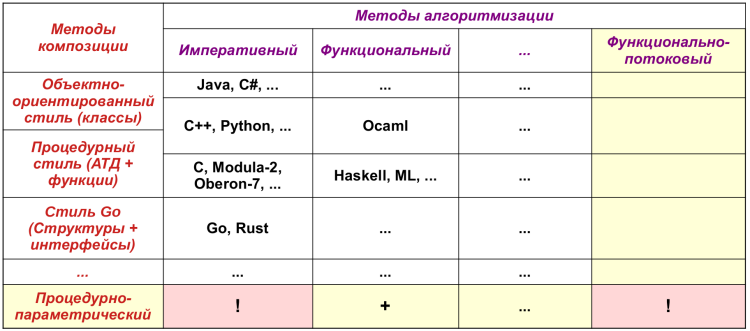
\includegraphics[width=1.0\textwidth]{img/f02-01.png}
    \caption{Классификация языков по методам алгоритмизации и методам композиции}
    \label{f02-01}
\end{figure}


% --- Методы задания однозначности и их отражение в архитектурах ВС ---
% Методы задания однозначности и их отражение в архитектурах ВС

\chapter{Методы задания однозначности и их отражение в архитектурах ВС}

Одним из ключевых моментов многоуровневой организации архитектур является подход к определению однозначности операций выполняемых, компьютером. Под однозначностью в данном случае понимается четкое понимание того, какие данные какого типа поступают на вход операции и какой получается тип результата после ее выполнения. Данный вопрос непосредственно связан с представлением типов в языках программирования~\cite{types-in-prog-lang} и подходами к их использованию. Более детально эти вопросы исследуются теорией типов~\cite{types-theory}.

\section{Пример неоднозначной трактовки алгоритма}

Основные проблемы, с заданием однозначности можно рассмотреть на весьма простом примере, связанным с созданием алгоритмов на начальном этапе их изучения. Обычно в рамках этого процесса используется некоторый упрощенный язык описания алгоритмов и представляется архитектура исполнителя. Выберем в качестве представления словесное описание алгоритма с использованием следующих команд:

\begin{verbatim}
    1. Начало
    2. Конец
    3. Ввод
    4. Вывод
    5. Операция
    6. Условный переход
    7. Безусловный переход
\end{verbatim}
Данные команды вполне понятны на интуитивном уровне и позволяют разрабатывать <<программы>> для компьютера обобщенная схема которого представлена на рисунке~\ref{type-01}.
\begin{figure}[htbp]
    \centering
    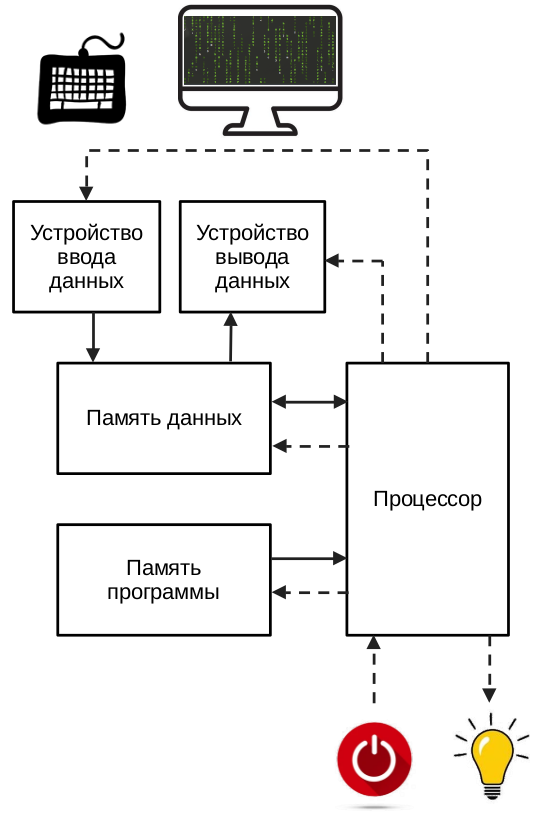
\includegraphics[width=0.4\textwidth]{img/type-01.png}
    \caption{Обобщенная архитектура простейшего исполнителя алгоритмов}
    \label{type-01}
\end{figure}
Алгоритм записывается в память программы. Данные размещаются соответственно в памяти данных. Есть некоторый ввод данных, а также вывод формируемых результатов. Операции выполняет процессор. Запуск программы осуществляется нажатием кнопки пользователем. При завершении выполнения программы загорается лампочка. В принципе на интуитивном уровне достаточно понятно как функционирует такая система.

Рассмотрим, каким образом будет выполняться на такой системе программа вычисления факториала:

\begin{ffcode}
0. Начало
1. Ввод N
2. F = 1
3. Если N < 2 На 7
4. F = F * N
5. N = N - 1
6. На 3
7. Вывод F
8. Конец
\end{ffcode}

Для имитации выполнения можно использовать ручной метод прокрутки для некоторых исходных данных. После загрузки программы наша система будет находиться в ожидании запуска (рисунок~\ref{type-02}).
\begin{figure}[htbp]
    \centering
    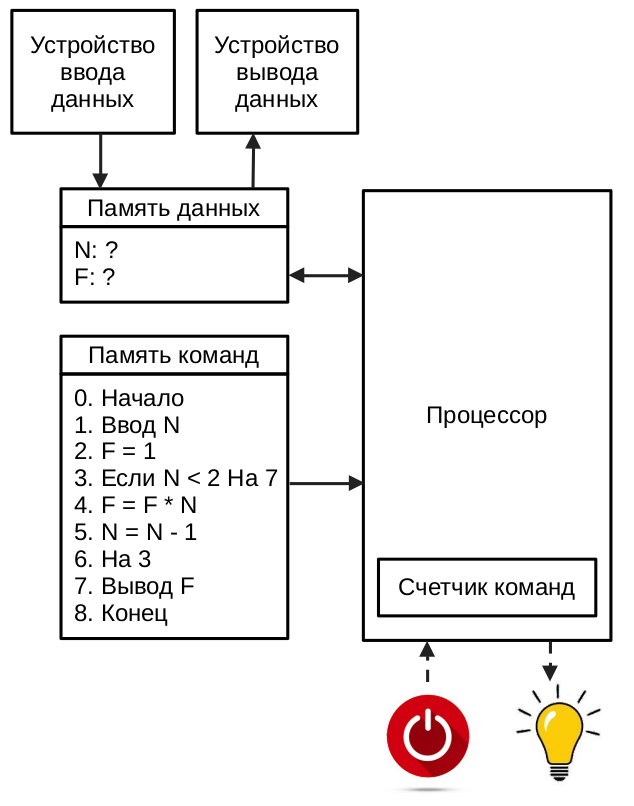
\includegraphics[width=0.4\textwidth]{img/type-02.png}
    \caption{Обобщенная архитектура простейшего исполнителя алгоритмов}
    \label{type-02}
\end{figure}
После нажатия на кнопку запуска программы система ищет начальную команду, устанавливая счетчик команд в нулевое значение (рисунок~\ref{type-03}). Затем осуществляется переход в автоматический режим с переключение на следующую команду счетчика команд.
\begin{figure}[htbp]
    \centering
    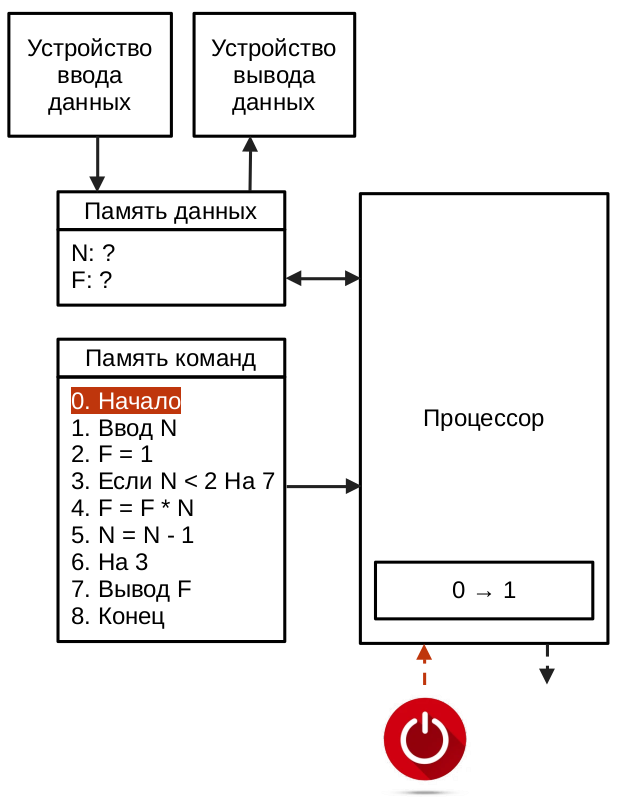
\includegraphics[width=0.4\textwidth]{img/type-03.png}
    \caption{Обобщенная архитектура простейшего исполнителя алгоритмов}
    \label{type-03}
\end{figure}
Выполнение команды ввода в команде 1 позволяет получить значение операнда N (рисунок~\ref{type-04}).
\begin{figure}[htbp]
    \centering
    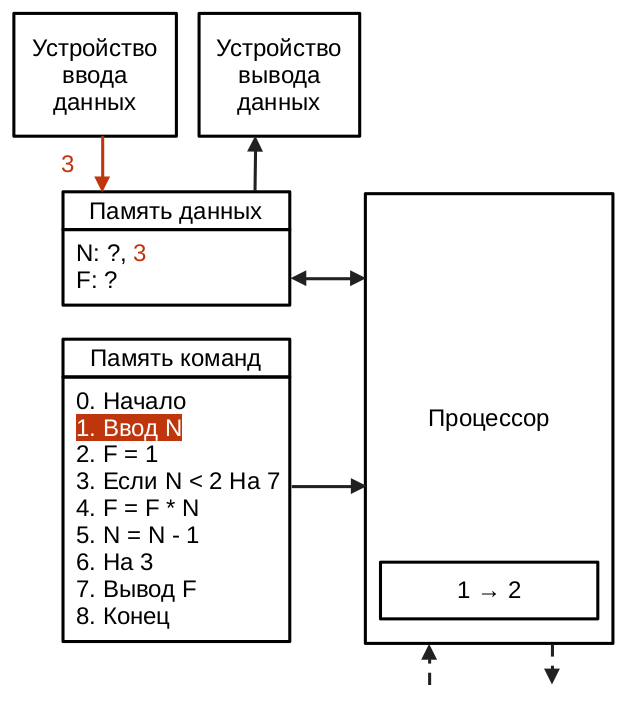
\includegraphics[width=0.4\textwidth]{img/type-04.png}
    \caption{Обобщенная архитектура простейшего исполнителя алгоритмов}
    \label{type-04}
\end{figure}

\begin{figure}[htbp]
    \centering
    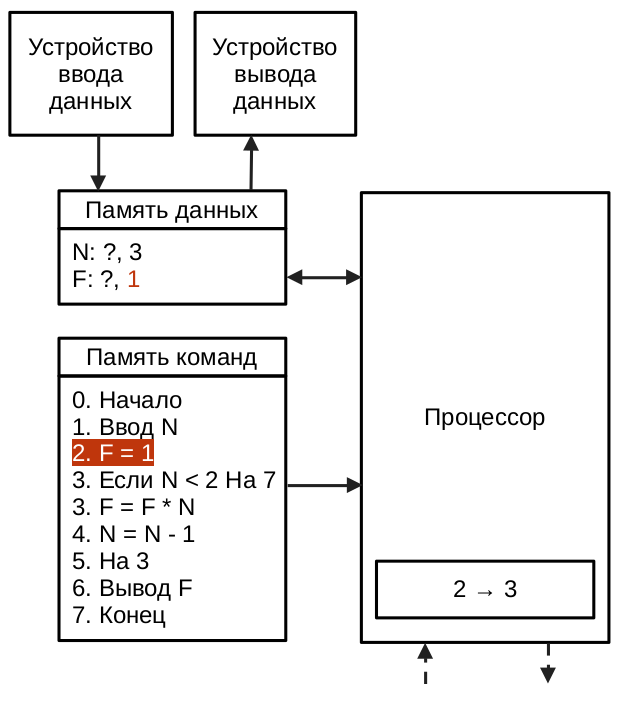
\includegraphics[width=0.4\textwidth]{img/type-05.png}
    \caption{Обобщенная архитектура простейшего исполнителя алгоритмов}
    \label{type-05}
\end{figure}
Следующая команда присваивает переменной F значение, равное  1 (рисунок~\ref{type-05})

Дальнейшие вычисления выполняются в автоматическом режиме до выполнения команды завершения программы (рисунок~\ref{type-13}).
\begin{figure}[htbp]
    \centering
    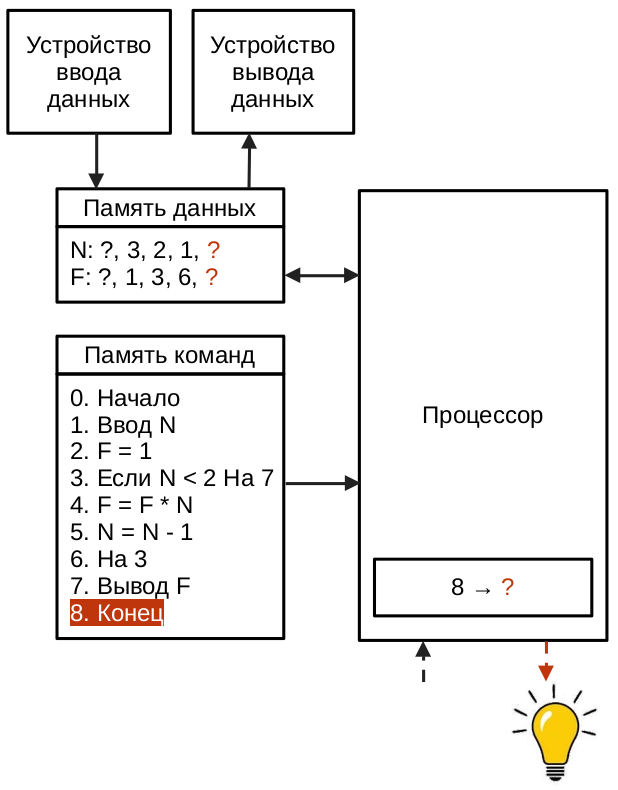
\includegraphics[width=0.4\textwidth]{img/type-13.png}
    \caption{Обобщенная архитектура простейшего исполнителя алгоритмов}
    \label{type-13}
\end{figure}

\textbf{примечание.}
\textit{Пока описано как есть. Возможно стоит описать более подробно все шаги и подставить все необходимые рисунки.}

Глядя на приведенный алгоритм и понимая его только на интуитивном уровне, человек может получить конечный результат, опираясь на свой опыт и знания даже в условиях неоднозначного представления информации. В частности, его мало волнуют следующие вопросы:
\begin{itemize}
    \item Можно ли использовать действительные числа, символы, строки?
	\item Как воспринимается ввод данных?
	\item Как отображаются данные?
	\item На какие устройства ввода-вывода можно использовать?
	\item Какова семантика каждой выполняемой операции?
	\item Какой тип памяти данных у N и F?
\end{itemize}
Возникает также вопрос: а может ли реальный компьютер выполнить данный алгоритм без наличия представленной выше информации?

Реализуем на языке программирования С аналогичную программу для компьютера и посмотрим, что изменилось.

\begin{ffcode}
#include <stdio.h>

static int n;
static int f = 1;

int main() {
  // Во время выполнения:
  printf("n? ");           // calc(char*)
  scanf("%d", &n);         // calc(char*); if(%d)-> use n as int
loop:
  // Во время компиляции:
  if(n < 2) goto end;      // <(int, int) -> bool
  f *= n;                  // *(int, int) -> int; =(int) -> int
  n--;                     // --(int) -> int
  goto loop;
end:
  // Во время выполнения:
  printf("n! = %d\n", f);  // calc(char*); if(%d)-> use n as int
}
\end{ffcode}
Мы видим, что появились описания типов данных, которые обеспечивают поддержку однозначности при выполнении операций. Любая выполняемая операция имеет полную информацию о своих аргументах, что позволяет однозначно сформировать тип и значения результата. Подобный контроль данных позволяет компьютеру не <<задумываться>> о том, с каким данными он работает. За него обо всем позаботился программист, предоставив всю необходимую информацию для компилятора.

Однако на самом деле не все так безоблачно, так как не всю информацию можно четко определить во время компиляции. Это касается вводимых в программу данных. Они вводятся в символьном виде и преобразуются во внутреннее представление на этапе вычислений. Следовательно корректность ввода и преобразования из вне во внутрь осуществляются компьютером и при некорректном вводе данных могут привести к неправильным результатам. Это говорит о том, что динамические трансформации и их контроль необходимы и в случае четкого контроля выполняемых действий. Данную программу легко сделать неправильной только изменением форматов для вводимых и (или) выводимых данных:

\begin{ffcode}
#include <stdio.h>

static int n;
static int f = 1;

int main() {
  // Во время выполнения:
  printf("n? ");            // calc(char*)
  scanf("%c", &n);          // calc(char*); if(%c)-> use n as char
loop:
  // Во время компиляции:
  if(n < 2) goto end;       // <(int, int) -> bool
  f *= n;                   // *(int, int) -> int; =(int) -> int
  n--;                      // --(int) -> int
  goto loop;
end:
  // Во время выполнения:
  printf("n! = %s\n", f);  // calc(char*); if(%s)-> use n as char*
}
\end{ffcode}

\section{Способы задания однозначности}

\textbf{Однозначность} определяет четкие правила выполнения операций реальными и виртуальными вычислительными системами, позволяя избегать или обходить ошибки программирования.

Различные методы задания однозначности операций позволяют контролировать корректность программы с разной степенью и на различных стадиях обработки 

Существуют различные виды однозначности, что напрямую связано с использованием типов в языках программирования:
\begin{enumerate}
    \item операционная однозначность (бестиповые системы);
    \item динамическая однозначность (системы с динамической типизацией);
    \item статическая однозначность (системы со статической типизацией).
\end{enumerate}
Также можно отметить, что в языках программирования обычно используются все подходы независимо от того, как позиционируется сам язык. Это отражается и на многоуровневую организацию архитектур ВС.

\subsection{Операционная однозначность}

Операционная однозначность, определяется через операции того или иного языка программирования, определяющего архитектуру реальной или виртуальной ВС. Она формируется за счет четкого определения что и с какими типами данных делает каждая операция. Сами данные при этом не несут никакой дополнительной информации о своем типе и рассматриваются в виде совокупности байт (бит), размещенных в памяти. Доступ к обезличенным данным осуществляется по адресам, задаваемым в операциях. Для таких архитектур характерны бестиповые языки.

Примеры подобных архитектур:
\begin{itemize}
    \item современные (традиционные) архитектуры уровня системы команд и их языки ассемблера;
    \item объектно-ориентированный язык программирования Eolang (и архитектура его виртуальной машины);
    \item частичная поддержка в языках системного программирования.
\end{itemize}

Реализаци бестипового программирования обычно осуществляется на уровне системы команд, характерном практически для всех существующих архитектур ВС. Каждая команда определяет операцию над обезличенными данным с учетом специфики той или иной архитектуры и реализации языка Ассемблера. Например, низкоуровневая программа, написанная с использованием Gnu Assembler и библиотеки \code{libc} будет выглядеть следующим образом:

\begin{ffcode}
# asm-fact.s
    .intel_syntax noprefix
# Константные данные
    .section  .rodata
question:
    .string "n? "
    .equ    questionLength, .-question-1
formatIn:
    .string "%d"
    .equ    formatInLength, .-formatIn-1
formatOut:
    .string "n! = %d\n"
    .equ    formatOutLength, .-formatOut-1

# Статические переменные
    .data
n:  .long   0

# Текст программы
    .text
    .globl  main
main:
    push    rbp                     # пролог
    mov     rbp, rsp

    # Ввод начального значения n
    lea     rdi, question[rip]      # адрес формата подсказки
    mov     eax, 0                  # не действительные числа
    call    printf@plt              # печать подсказки

    lea     rdi, formatIn[rip]      # адрес формата числа
    lea     rsi, n[rip]
    mov     eax, 0                  # не действительные числа
    call    scanf@plt               # ввод целого

    # Вычисление факториала
    mov     eax, 1                  # начальная установка f
    mov     ebx, n[rip]             # перенос n в регистр
loop:
    cmp     ebx, 2                  # проверка на завершение
    jl      end                     # выход по меньше
    mul     ebx                     # f *= n
    dec     ebx                     # --n;
    jmp     loop
end:

    # Вывод результата вычислений
    lea     rdi, formatOut[rip]     # адрес формата результата
    mov     rsi, rax                # значение результата
    mov     eax, 0                  # не действительные числа
    call    printf@plt              # печать результата

    mov     eax, 0                  # return 0
    pop     rbp                     # эпилог
    ret
\end{ffcode}

Использование бестипового программирования не обязательно рассматривать на языках уровня системы команд. Необходимость эффективной манипуляции с компьютерной памятью ведет к тому, что в языках системного программирования используются конструкции, позволяющие легко писать бестиповой код. Поэтому программу, осуществляющую вычисление факториала можно представить следующим образом:

\begin{ffcode}
#include <stdio.h>

static char memory[2*sizeof(int)];     // Память для n и f
static void* n = memory;               // Адрес на область для n
static void* f = memory + sizeof(int); // Адрес на область для f

int main() {
    *((int*)f) = 1;
    printf("n? ");
    scanf("%d", n);
    printf("n = %d\n", *((int*)n));
    printf("f = %d\n", *((int*)f));
loop:
    if(*((int*)n) < 2) goto end;
    *((int*)f) *= *((int*)n);
    (*(int*)n)--;
    goto loop;
end:
    printf("n! = %d\n", (*(int*)f));
}
\end{ffcode}
Отображение на компьютерную память в данном случае осуществляется с использованием символьного массива, обеспечивающего резервирование в ней соответствующего числа байт. Адреса в этомй памяти для \code{n} и \code{f} фиксируются через соответствующие указатели. Для того, чтобы операции языка C имели информацию об обрабатываемых ими типах данных, необходимо явным образом осуществить их приведение к нужном типу. Это приведение возлагается на программиста, что может вести к ошибкам при написании больших программ в бестиповом стиле.

\subsection{Динамическая однозначность}

Динамическая однозначность операций формируется за счет того, что с каждым значением, формируемым в программе сопоставляется его тип. Любая операция над данным может проверить этот тип и выбрать в соответствии с этим нужные вычисления. То есть, одна и та же операция может обрабатывать различные типы данных. При этом идентификация типа осуществляется во время выполнения программы. Одни и те же переменные могут хранить данные различного типа. В любой момент программа может проверить тип переменной. Данный подход широко используется в языках программирования, ориентированных на интерпретацию.

Примеры подобных архитектур:
\begin{itemize}
    \item Языки сценариев: Python, JavaScript, Lua и~др.;
    \item Языки функционального программирования: Lisp и~др.
\end{itemize}
Следует отметить, что в настоящее время практически отсутствую аппаратные решения, ориентированные на поддержку динамической однозначности. Хотя одно время (до эпохи сверхбольших интегральных схем) существовали несколько проектов~\cite{modern-arch}. В качестве примера можно отметить процессор фирмы Intel iAPX~432~\cite{i432-1,i432-2}.


\subsection{Статическая однозначность}

\textbf{Статическая однозначность} операций формируется за счет того, что с каждым значением в программе сопоставляется его тип. Этот тип задается при описании переменных и может быть проверен во время компиляции. Для всех временных и промежуточных значений тип может быть также выведен во время компиляции. Поэтому его не имеет смысла проверять во время выполнения. Одна и та же операция может быть задана с разными типами, но все вопросы по ее конкретному выполнению решаются во время компиляции (статический полиморфизм). С каждой переменной сопоставляется только один тип.Допускает эффективную трансформацию в бестиповые архитектуры уровня системы команд. Используется в языках компилируемого типа.

Примеры подобных архитектур:
\begin{itemize}
    \item Императивные языки программирования:C, C++, Pascal, Oberon family, Java, C\#, Rust, Go и~др;
    \item Языки функционального программирования: ML, Haskell и~др.
\end{itemize}
Из-за возможностей эффективной компиляции статически типизируемых программ в бестиповые практически отсутствует необходимость в разработке аппаратных решений для таких архитектур. Однако понимание, каким образом в ходе компиляции происходят трансформации из одной архитектуры в другую необходимы в связи с распространенностью языков со статической типизацией, обеспечивающих при программировании наиболее высокую надежность ПО за счет тотального контроля на этапе компиляции.

Завершая данный раздел следует отметить, что в разных частях больших программ мог могут применяться различные решения, что определяется как особенностью решаемой задачи, так и спецификой используемого языка программирования. В частности, при обработке данных альтернативных типов приходится моделировать их динамическую проверку за счет использования специальных тегов. Для передачи произвольных данных в функции языки C и C++ предоставляют указатель на \code{void}, который обеспечивает поддержку бестипового программирования.
% --- Представление данных ---
\chapter{Представление данных в вычислительных системах}



\section{Представление целочисленных данных}

В этом разделе описываются два разных способа использования битов для представления целых чисел: один из этих способов позволяет представлять только неотрицательные числа, а другой --- отрицательные числа, положительные и ноль. Позже мы увидим, что они сильно взаимосвязаны как математическими свойствами, так и реализациями на машинном уровне. Мы также рассмотрим влияние расширения или сжатия целых чисел, чтобы их можно было уместить в представления с разной длиной.

\subsection{Представление целых без знака}

Пусть имеется целочисленный тип, представляющий значения из w бит. Битовый вектор записывается либо как $\vec{x}$, что обозначает вектор как единое целое, либо как $[x_{n-1}, x_{n-2}...x_0]$ с перечислением отдельных битов в векторе. Рассмотрим $\vec{x}$ как число, записанное в двоичном виде. В этом случае мы получим интерпретацию $\vec{x}$ как числа без знака. Каждый бит $x_i$ имеет значение 0 или 1. В последнем случае он соответствует величине $2^i$, которая является составной частью всего числа.



\section{Представление значений с плавающей точкой. Cтандарт IEEE}

Позиционное представление, подобное рассмотренному в предыдущем разделе, неэффективно для очень больших чисел. Например, представление $5 × 2^{100}$ будет состоять из комбинации битов 101, за которой следует 100 нулей. Вместо этого предпочтительнее представлять такие числа в форме $x × 2^y$ путем задания значений х и y.

Стандарт IEEE определяет представление чисел с плавающей точкой в виде:
\begin{center}
    \large{$V = (-1)^s × M × 2^E$}
\end{center}
где:
\begin{itemize}
    \item символ $s$ определяет знак числа, который может быть отрицательным при $s = 1$ или положительным при $s = 0$ (интерпретация знакового разряда для числового значения 0 рассматривается как особый случай);
    \item мантисса М --- дробное двоичное число в диапазоне от 1 до 2 – $\varepsilon$ или от 0  до 1 – $\varepsilon$ (значение $\varepsilon$ определяет точность вычислений и зависит от разрядности мантиссы);
    \item показатель Е – взвешивает величину (возможно, отрицательной)  степенью 2.
\end{itemize}

Для кодировки этих величин битовое представление числа с плавающей точкой делится на три поля:

\begin{itemize}
    \item знаковый бит s напрямую кодирует символ s;
    \item k-разрядное поле показателя $ехр = e_{k-1} ... e_1e_0$ кодирует показатель Е;
    \item n-разрядное поле дробной части $frac = f_{n-1} ... f_1f_0$ кодирует мантиссу М, способ кодирования также зависит от того, равно поле показателя 0 или нет.
\end{itemize}

На рис~\ref{data01}. 2.13 показано, как эти три поля упакованы в два наиболее распространенных формата. В формате с одинарной точностью (тип float в языке С) поля s, exp и frac имеют размеры 1, k = 8 и n = 23 бит, что дает 32-разрядное представление. В формате с двойной точностью (тип double в языке С) поля s, ехр и frac имеют размеры 1, k = 11, n = 52 бит, что дает 64-разрядное представление.

\begin{figure}[htbp]
    \centering
    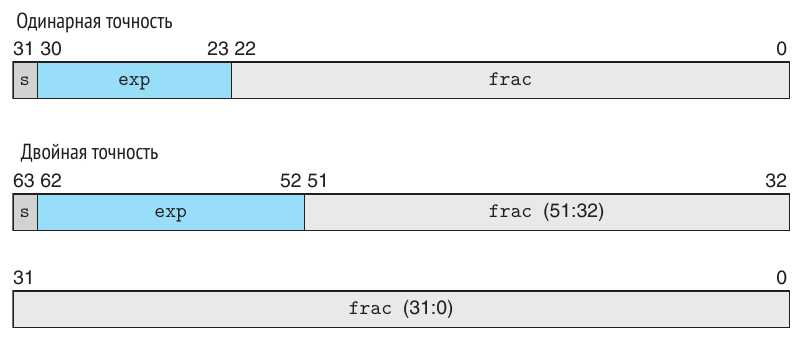
\includegraphics[width=0.8\textwidth]{img/data01.png}
    \caption{Стандартные форматы представления чисел с плавающей запятой}
    \label{data01}
\end{figure}

Величину, представленную конкретным битовым представлением, можно разделить на три разных варианта (последний имеет два подварианта), в зависимости от значения ехр. Они показаны на рисунке~\ref{data02}.

\begin{figure}[htbp]
    \centering
    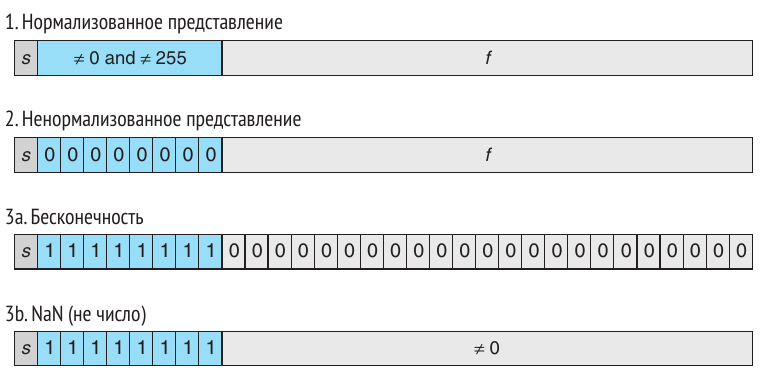
\includegraphics[width=0.8\textwidth]{img/data02.png}
    \caption{Категории значений с плавающей запятой одинарной точности. Значение показателя определяет, является число (1) нормализованным, (2) ненормализованным или (3) особым}
    \label{data02}
\end{figure}

\subsection{Вариант 1: нормализованные значения}

Это самый общий случай. Он имеет место, когда комбинация битов ехр состоит либо из одних нулей (числовое значение 0), либо из одних единиц (числовое значение 255 для одинарной точности и 2047 для двойной). В этом случае поле показателя интерпретируется как целое со знаком в смещенной форме. То есть показатель имеет значение $Е = е - Bias$ (смещение), где $е$ – число без знака с битовым представлением $e_{k-1} ... e_1e_0$, a $Bias$ --- величина смещения, равная $2^{k-1} - 1$ (127 для одинарной точности, 1023 --- для двойной). Это разложение дает диапазон показателей от -126 до +127 для одинарной точности и от -1022 до +1023 – для двойной.

Поле дробной части frac интерпретируется как представляющее дробную величину f, где $0 \leq f < 1$, имеющую двоичное представление $0.f_{n-1} ... f_1f_0$, т.~ е. с двоичной точкой слева от самого значимого бита. Мантисса определяется как $М = 1 + f$. Иногда такое представление называют представлением с неявной ведущей единицей, потому что M можно рассматривать как число с двоичным представлением $1.f_{n-1}f{n-2} ... f_0$. Такое представление позволяет получить дополнительный бит точности, поскольку показатель Е всегда можно настроить так, чтобы мантисса М находилась в диапазоне $1 \leq M < 2$ (при условии отсутствия переполнения). Поэтому нет необходимости явно представлять ведущий, так как он всегда равен единице.

\begin{center}
\framebox[\textwidth][l]{
\begin{minipage}{0.95\linewidth}
\textbf{Зачем устанавливать смещение для ненормализованных значений}

Использование значения показателя 1 - Bias вместо простого -Bias может показаться противоречащим здравому смыслу. Но очень скоро вы увидите, что такое представление упрощает переход от ненормализованных значений к нормализованным.
\end{minipage}
}
\end{center}

\subsection{Вариант 2: ненормализованные значения}

Когда поле показателя состоит только из нулей, то представляемое число находится
в ненормализованной форме. В этом случае значение порядка Е = 1 - Bias, а значение мантиссы M = f, т. е. значение дробной части не имеет неявной ведущей единицы.

Ненормализованные значения служат двум целям. Во-первых, они позволяют представлять числовое значение 0, поскольку для нормализованного представления всегда выполняется условие $M \geq 1$, и, следовательно, оно не позволяет представить 0. Фактически представление чисел с плавающей точкой +0.0 имеет комбинацию битов, состоящую из одних нулей: знаковый разряд содержит 0, поле показателя
полностью состоит из нулей (что указывает на ненормализованное значение), и поле дробной части тоже состоит из одних нулей, давая M = f = 0. Интересно, что когда знаковый разряд равен единице, а все другие поля – нулю, то получается значение -0.0. В формате IEEE с плавающей точкой значения -0.0 и +0.0 в одних случаях
рассматриваются как разные, а в других – как одинаковые.

Вторая цель, которую преследуют ненормализованные значения, – представление чисел, близких к 0.0. Они обеспечивают свойство равномерного приближения к нулю, при котором возможные числовые значения равномерно располагаются около 0.0.

\subsection{Вариант 3: особые значения}

Последняя форма представления значений используется, когда поле показателя со
стоит из одних единиц. Если при этом поле дробной части состоит из одних нулей, то в результате получается бесконечность: либо $+\infty$, когда s = 0, либо $-\infty$, когда s = 1. Бесконечность может представлять переполнение как при умножении очень больших чисел, так и при делении на ноль. Когда дробная часть не равна нулю, то такое значение называется NaN (сокращенно <<Not a Number>> – не число). Такие значения возвращаются, когда результат операции нельзя представить вещественным числом или бесконечностью, как, например, $\sqrt{-1}$ или $\infty - \infty$. Они также могут пригодиться в некоторых приложениях для инициализации данных.

% --- Архитектуры уровня системы команд. Общие характеристики ---
% --- Архитектура процессоров семейства RISC-V ---
\chapter{Архитектура процессорв семейства RISC-V}

\section{Особенности семейства RISC-V}

Принципы RISC:
\begin{itemize}
    \item отсутствие вычислительно сложных инструкций;
    \item фиксированная длина инструкции;
    \item большое количество регистров общего назначения;
    \item ограничения на работу непосредственно с оперативной памятью как с медленным устройством.
\end{itemize}


\section{Форматы команд}

Процессор содержит:
\begin{itemize}
    \item 32 регистра общего назначения, доступа к специализированным регистрам нет (в т. ч. нет регистра флагов, даже на аппаратном уровне!);
    \item 4 базовых типа команд (рисунок~\ref{command-01}):
    \begin{itemize}
        \item \textbf{R} --- типа «регистр-регистр-регистр» (Register)
        \item \textbf{I} --- типа «непосредственное значение-регистр-регистр» (Immediate)
        \item \textbf{S} --- типа «регистр-регистр-непосредственное значение» (Store)
        \item \textbf{U} --- типа «непосредственное значение-регистр» (Upper)
    \end{itemize}
    \item
    \item
    \item
    \item
    \item
\end{itemize}

\begin{figure}[htbp]
    \centering
    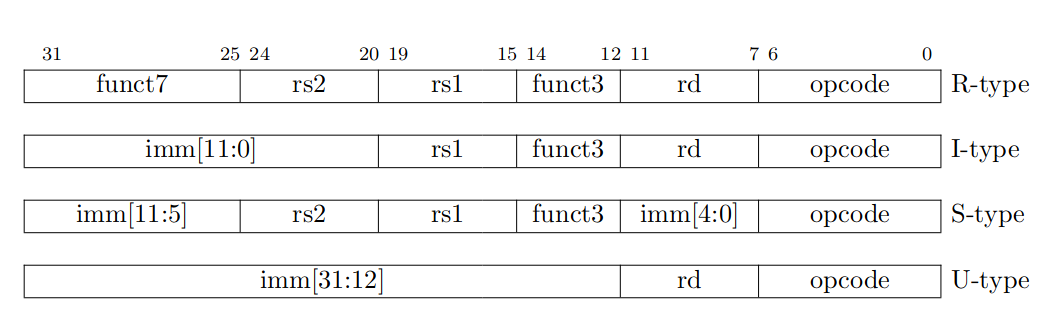
\includegraphics[width=1.0\textwidth]{img/RISCV_4_Commands.png}
    \caption{Основные форматы команд 32-разрядного процессора RISC-V}
    \label{command-01}
\end{figure}
Обозначения на рисунке:
\begin{itemize}
    \item \textbf{opcode} — код операции (6 битов)
    \item \textbf{rs1} --- № регистра-источника (5 битов)
    \item \textbf{rs2} --- № регистра-опреанда (5 битов)
    \item \textbf{rd} --- № регистра-приёмника (5 битов)
    \item \textbf{imm[11:0]} --- непосредственный операнд размером в 12 битов (В случае, когда непосредственное значение определяет «приёмник» (смещен адреса для «близкого» перехода или записи результата в память), 12 битов целиком в поле rd не помещаются, и его приходится «распиливать» (инструкция типа S). Непосредственный операнд всегда знаковый, и его знак всегда приходится на 31-й бит)
    \item \textbf{imm[31:12]} --- непосредственный операнд размером в 20 битов. Используется в инструкциях типа U для заполнения старших двадцати битов регистра (в операциях «далёкого» перехода и как дополнительная инструкция при записи в регистр полного 32-разрядного непосредственного операнда)
    \item \textbf{funct} --- поле функции (6 битов), используется для разных инструкций, у которых код операции одинаковый. Например, все арифметические инструкции типа I имеют одинаковый opcode OP-IMM (чему он равен?), а различаются полем funct. По-видимому, для эффективной реализации R-команд в конвейере удобнее не декодировать опкод, а по-быстрому сравнить его с нулём, и получать значения регистров, параллельно декодируя функцию, чтобы потом её применить.
\end{itemize}

\debate[Примечание]{Ниже представлен альтернативных рисунок из Reference Card с большим числом форматов. На всякий случай. Просто ряд форматов имеют одинаковые поля, но различную семантику. Пока непонятно, что лучше и проще преподносить. Может сказать о второй форме как способ уточнения семантики?}

Щесть базовых типов команд (рисунок~\ref{command-02}):

\begin{figure}[htbp]
    \centering
    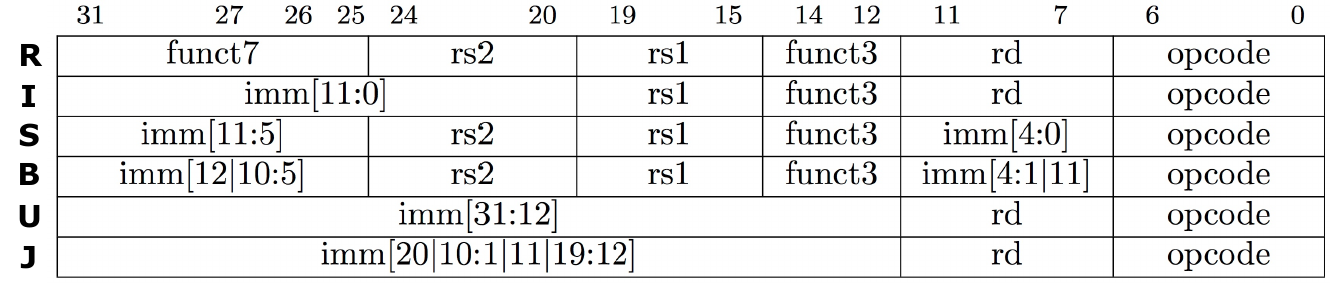
\includegraphics[width=1.0\textwidth]{img/32-bit-instruction-formats.png}
    \caption{Основные форматы команд 32-разрядного процессора RISC-V}
    \label{command-02}
\end{figure}

\section{Базовый набор команд процессора}

Процессор содержит основной набор команд, каждая из который отображается в одну инструкцию на языке ассемблера. Вместе с тем ассемблер, для повышения удобства программирования, дополнительно поддерживает псевдокоманды, каждая из которых может кодировать до нескольких машинных команд или иметь специфические операнды, позволяющие сформировать мнемонику команды, удобную для восприятия человеком.

Арифметические команды представлены в таблице~\ref{table-base-arithmetic}

\begin{table}[h]
    \caption{Арифметические команды набора RV32I}
    \centering
    \begin{tabularx}{\textwidth}{|l|c|X|}
        \hline
        \textbf{Команда} & \textbf{Формат} & \textbf{Описание} \\
        %\hline  \multicolumn{3}{|c|}{\textbf{\textit{Арифметические}}} \\
        \hline \verb|add rd,rs1,rs2| & R & Целочисленное сложение: \verb|rd  = rs1 + rs2| \\
        \hline \verb|addi rd,rs1,int12| & I & Сложение непосредственно с числом: \verb|rd = rs1 + int12| \\
        \hline \verb|sub t1,t2,t3| & R & Subtraction: set t1 to (t2 minus t3) \\
        \hline \verb|lui t1,100000| & U & Load upper immediate: set t1 to 20-bit followed by 12 0s \\
        \hline \verb|auipc rd,100000| & U & Сложение старших 20 разрядов непосредственного числа с \verb|pc|: \verb|rd = pc + int[31:12]| (pc плюс 20-бит непосредственного операнда как старшие разряды 32-разрядного числа, расширенного нулями) \\
        \hline
    \end{tabularx}
    \label{table-base-arithmetic}
\end{table}

Логические команды представлены в таблице~\ref{table-base-logical}

\begin{table}[h]
    \caption{Логические команды набора RV32I}
    \centering
    \begin{tabularx}{\textwidth}{|l|c|X|}
        \hline
        \textbf{Команда} & \textbf{Формат} & \textbf{Описание} \\
        %\hline  \multicolumn{3}{|c|}{\textbf{\textit{Арифметические}}} \\
        \hline \verb|add rd,rs1,rs2| & R & Целочисленное сложение: \verb|rd  = rs1 + rs2| \\
        \hline \verb|addi rd,rs1,int12| & I & Сложение непосредственно с числом: \verb|rd = rs1 + int12| \\
        \hline \verb|sub t1,t2,t3| & R & Subtraction: set t1 to (t2 minus t3) \\
        \hline \verb|lui t1,100000| & U & Load upper immediate: set t1 to 20-bit followed by 12 0s \\
        \hline
    \end{tabularx}
    \label{table-base-logical}
\end{table}


Команды сдвига представлены в таблице~\ref{table-base-shift}

\begin{table}[h]
    \caption{Команды сдвига набора RV32I}
    \centering
    \begin{tabularx}{\textwidth}{|l|c|X|}
        \hline
        \textbf{Команда} & \textbf{Формат} & \textbf{Описание} \\
        \hline \verb|xor t1,t2,t3| & R & Bitwise XOR : Set t1 to bitwise XOR of t2 and t3 \\
        \hline \verb|xori t1,t2,-100| & I & Bitwise XOR immediate : Set t1 to bitwise XOR of t2 and sign-extended   12-bit immediate \\
        \hline \verb|or t1,t2,t3| & R & Bitwise OR : Set t1 to bitwise OR of t2 and t3 \\
        \hline \verb|ori t1,t2,-100| & I & Bitwise OR immediate : Set t1 to bitwise OR of t2 and sign-extended 12-bit immediate \\
        \hline \verb|and rd,rs1,rs2| & R & Поразрядное И: \verb|rd = rs1 & rs2| \\
        \hline \verb|andi rd,rs1,int12| & I & Поразрядное И непосредственно с числом: \verb|rd = rs2 & int12| (с расширением знакового разряда у int12) \\
        \hline
    \end{tabularx}
    \label{table-base-shift}
\end{table}

Команды сравнения представлены в таблице~\ref{table-base-compare}

\begin{table}[h]
    \caption{Команды сравнения набора RV32I}
    \centering
    \begin{tabularx}{\textwidth}{|l|c|X|}
        \hline
        \textbf{Команда} & \textbf{Формат} & \textbf{Описание} \\
        \hline \verb|slt t1,t2,t3| & R & Set less than : If t2 is less than t3, then set t1 to 1 else set t1 to 0 \\
        \hline \verb|slti t1,t2,-100| & I & Set less than immediate : If t2 is less than sign-extended 12-bit immediate, then set t1 to 1 else set t1 to 0 \\
        \hline \verb|sltu t1,t2,t3| & R & Set less than : If t2 is less than t3 using unsigned comparision, then set t1 to 1 else set t1 to 0 \\
        \hline \verb|sltiu t1,t2,-100| & I & Set less than immediate unsigned : If t2 is less than sign-extended 16-bit immediate using unsigned comparison, then set t1 to 1 else set t1 to 0 \\
        \hline
    \end{tabularx}
    \label{table-base-compare}
\end{table}

Команды ветвления представлены в таблице~\ref{table-base-branch}

\begin{table}[h]
    \caption{Команды ветвления набора RV32I}
    \centering
    \begin{tabularx}{\textwidth}{|l|c|X|}
        \hline
        \textbf{Команда} & \textbf{Формат} & \textbf{Описание} \\
        \hline \verb|beq t1,t2,label| & B & Переход, если равно: Переход к оператору по label, если \verb|t1 == t2|. \\
        \hline \verb|bge t1,t2,label| & B & Перейти, если больше или равно: перейти к оператору по label, если \verb|t1 >= t2| \\
        \hline \verb|bgeu t1,t2,label| & B & Переход, если больше или равно для беззнаковых чисел: переход к оператору по адресу метки, если \verb|t1 >= t2| (с беззнаковой интерпретацией)  \\
        \hline \verb|blt t1,t2,label| & B & Переход, если меньше: Переход к оператору по label, если \verb|t1 < t2| \\
        \hline \verb|bltu t1,t2,label| & B & Переход, если меньше для беззнаковых чисел: переход к оператору по label, если \verb|t1 < t2| (с беззнаковой интерпретацией) \\
        \hline \verb|bne t1,t2,label| & B & Переход, если не равно: Переход к оператору по label, если \verb|t1 != t2|. \\
        \hline
    \end{tabularx}
    \label{table-base-branch}
\end{table}

Команды перехода и связывания представлены в таблице~\ref{table-base-jump}

\begin{table}[h]
    \caption{Команды перехода и связывания набора RV32I}
    \centering
    \begin{tabularx}{\textwidth}{|l|c|X|}
        \hline
        \textbf{Команда} & \textbf{Формат} & \textbf{Описание} \\
        \hline \verb|jal t1, target| & J & Jump and link : Set t1 to Program Counter (return address) then jump to statement at target address \\
        \hline \verb|jalr t1, t2, -100| & I & Jump and link register: Set t1 to Program Counter (return address) then jump to statement at t2 + immediate \\
        \hline
    \end{tabularx}
    \label{table-base-jump}
\end{table}

Команды синхронизации представлены в таблице~\ref{table-base-sync}

\begin{table}[h]
    \caption{Команды синхронизации набора RV32I}
    \centering
    \begin{tabularx}{\textwidth}{|l|c|X|}
        \hline
        \textbf{Команда} & \textbf{Формат} & \textbf{Описание} \\
        \hline \verb|fence 1, 1| & I & Ensure that IO and memory accesses before the fence happen before the following IO and memory accesses as viewed by a different thread \\
        \hline \verb|fence.i| & I & Ensure that stores to instruction memory are visible to instruction fetches \\
        \hline
    \end{tabularx}
    \label{table-base-sync}
\end{table}

Команды взаимодействия с окружением представлены в таблице~\ref{table-base-env}

\begin{table}[h]
    \caption{Команды взаимодействия с окружением набора RV32I}
    \centering
    \begin{tabularx}{\textwidth}{|l|c|X|}
        \hline
        \textbf{Команда} & \textbf{Формат} & \textbf{Описание} \\
        \hline \verb|ebreak| & I & Pause execution \\
        \hline \verb|ecall| & I & Issue a system call: Execute the system call specified by value in a7 \\
        \hline
    \end{tabularx}
    \label{table-base-env}
\end{table}

Команды работы с регистром состояния представлены в таблице~\ref{table-base-env}

\begin{table}[h]
    \caption{Команды работы с регистром состояния набора RV32I}
    \centering
    \begin{tabularx}{\textwidth}{|l|c|X|}
        \hline
        \textbf{Команда} & \textbf{Формат} & \textbf{Описание} \\
        \hline \verb|csrrc t0, fcsr, t1| & I & Atomic Read/Clear CSR: read from the CSR into t0 and clear bits of the CSR according to t1 \\
        \hline \verb|srrci t0, fcsr, 10| & I & Atomic Read/Clear CSR Immediate: read from the CSR into t0 and clear bits of the CSR according to a constant \\
        \hline \verb|csrrs t0, fcsr, t1| & I & Atomic Read/Set CSR: read from the CSR into t0 and logical or t1 into the CSR \\
        \hline \verb|csrrsi t0, fcsr, 10| & I & Atomic Read/Set CSR Immediate: read from the CSR into t0 and logical or a constant into the CSR \\
        \hline \verb|csrrw t0, fcsr, t1| & I & Atomic Read/Write CSR: read from the CSR into t0 and write t1 into the CSR \\
        \hline \verb|csrrwi t0, fcsr, 10| & I & Atomic Read/Write CSR Immediate: read from the CSR into t0 and write a constant into the CSR \\
        \hline
    \end{tabularx}
    \label{table-base-env}
\end{table}

Команды загрузки данных представлены в таблице~\ref{table-base-load}

\begin{table}[h]
    \caption{Команды загрузки данных набора RV32I}
    \centering
    \begin{tabularx}{\textwidth}{|l|c|X|}
        \hline
        \textbf{Команда} & \textbf{Формат} & \textbf{Описание} \\
        \hline \verb|lb t1, -100(t2)| & I & Set t1 to sign-extended 8-bit value from effective memory byte address \\
        \hline \verb|lbu t1, -100(t2)| & I & Set t1 to zero-extended 8-bit value from effective memory byte address \\
        \hline \verb|lh t1, -100(t2)| & I & Set t1 to sign-extended 16-bit value from effective memory halfword address \\
        \hline \verb|lhu t1, -100(t2)| & I & Set t1 to zero-extended 16-bit value from effective memory halfword address \\
        \hline \verb|lw t1, -100(t2)| & I & Set t1 to contents of effective memory word address \\
        \hline
    \end{tabularx}
    \label{table-base-load}
\end{table}

Команды выгрузки данных представлены в таблице~\ref{table-base-store}

\begin{table}[h]
    \caption{Команды выгрузки данных набора RV32I}
    \centering
    \begin{tabularx}{\textwidth}{|l|c|X|}
        \hline
        \textbf{Команда} & \textbf{Формат} & \textbf{Описание} \\
        \hline \verb|sb t1, -100(t2)| & S & Store byte : Store the low-order 8 bits of t1 into the effective memory byte address \\
        \hline \verb|sh t1, -100(t2)| & S & Store halfword : Store the low-order 16 bits of t1 into the effective memory halfword address \\
        \hline \verb|sw t1, -100(t2)|& S & Store word : Store contents of t1 into effective memory word address \\
        \hline
    \end{tabularx}
    \label{table-base-store}
\end{table}

Команды умножения, деления, выделения остатка, расширяющие базовый набор, и используемые в эмулятора RARS, представлены в таблице~\ref{table-base-mul}

\begin{table}[h]
    \caption{Команды умножения, деления, вычисления остатка набора RV32I}
    \centering
    \begin{tabularx}{\textwidth}{|l|c|X|}
        \hline
        \textbf{Команда} & \textbf{Формат} & \textbf{Описание} \\
        \hline \verb|mul t1,t2,t3| & R & Multiplication: set t1 to the lower 32 bits of t2*t3 \\
        \hline \verb|mulh t1,t2,t3| & R & Multiplication: set t1 to the upper 32 bits of t2*t3 using signed multiplication \\
        \hline \verb|mulhsu t1,t2,t3| & R & Multiplication: set t1 to the upper 32 bits of t2*t3 where t2 is signed and t3 is unsigned \\
        \hline \verb|mulhu t1,t2,t3| & R & Multiplication: set t1 to the upper 32 bits of t2*t3 using unsigned multiplication \\
        \hline \verb|div t1,t2,t3| & R & Division: set t1 to the result of t2/t3 \\
        \hline \verb|divu t1,t2,t3| & R & Division: set t1 to the result of t2/t3 using unsigned division \\
        \hline \verb|rem t1,t2,t3| & R & Remainder: set t1 to the remainder of t2/t3 \\
        \hline \verb|remu t1,t2,t3| & R & Remainder: set t1 to the remainder of t2/t3 using unsigned division \\
        \hline
    \end{tabularx}
    \label{table-base-mul}
\end{table}

Команды для работы по прерываниям представлены в таблице~\ref{table-base-mul}

\begin{table}[h]
    \caption{Команды для работы с прерываниями эмулятора RARS}
    \centering
    \begin{tabularx}{\textwidth}{|l|c|X|}
        \hline
        \textbf{Команда} & \textbf{Формат} & \textbf{Описание} \\
        \hline
        \hline \verb|uret| & ? & Return from handling an interrupt or exception (to uepc) \\
        \hline \verb|wfi| & ? & Wait for Interrupt \\
        \hline
    \end{tabularx}
    \label{table-base-instructions5}
\end{table}

Введенные обозначения:

int12 --- 12-разрядное целое со знаком

% --- Архитектура процессоров семейства ARM ---
\chapter{Архитектура процессорв семейства ARM}

\section{Особенности семейства ARM}

% --- Архитектура процессоров семейства Intel ---
\chapter{Архитектура процессорв семейства Intel}

\section{Особенности семейства Intel}

% --- Внутри функции main ---
% main. Внутри функции main

\chapter{Внутри функции main}

Как вы знаете, каждая программа на C начинается с выполнения функции с именем main, которая вызывается из функции запуска в среде выполнения C. Основная функция будет вызывать другие функции (подфункции) для выполнения большей части обработки. Даже простое <<\code{Hello, World!}>> программе необходимо вызвать другую функцию, чтобы вывести сообщение на экран.

Большинству подфункций требуется, чтобы данные передавались им в качестве аргументов от вызывающей функции, и они часто передают результат обратно вызывающей функции. Аргументами функции могут быть данные или адреса памяти. Когда функция вызывается, она выполняет свои операции, а затем возвращается к вызывающей функции. Вызывающая функция должна отправить вызываемой функции адрес для возврата. В архитектуре x86-64 адрес возврата передается в стеке вызовов.

Добавляя немного сложности, большинству функций нужны свои собственные локальные переменные для хранения данных и адресов. Регистры можно использовать для переменных, но они глобальны, и нам быстро не хватит регистров для использования. Стек обеспечивает хорошее место для выделения места для локальных переменных в памяти.

В этой главе мы разберем этот процесс. Мы сделаем это, обсудив, как писать символы на экране и читать символы с клавиатуры в нашей основной функции. Начиная с этой главы, мы обычно обходим функции стандартной библиотеки C, printf и scanf, и используем функции системного вызова write для вывода на экран и read для ввода с клавиатуры.

Мы начнем с обсуждения функций записи и чтения. Затем мы рассмотрим, как аргументы передаются функции в регистрах процессора. Далее мы рассмотрим, как ЦП может определить адрес для передачи функции, когда это необходимо. Затем мы рассмотрим, как структура данных, называемая стеком вызовов, используется для создания локальных переменных внутри функции.

\section{Функции системного вызова записи и чтения}

В главе 2 мы использовали \code{printf} и \code{scanf} из стандартной библиотеки C для записи на экран и чтения с клавиатуры. Как показано на рис. 2-1 (в главе 2), \code{printf} преобразует данные из формата хранения в памяти в символьный формат и вызывает функцию системного вызова \code{write} для отображения символов на экране. При чтении символов с клавиатуры \code{scanf} вызывает функцию системного вызова \code{read} и преобразует символы в формат хранения в памяти.

Linux видит экран и клавиатуру как файлы. При первом запуске программы операционная система открывает три файла — стандартный ввод, стандартный вывод и стандартный файл ошибок — и присваивает каждому файлу целое число, называемое файловым дескриптором. Программа взаимодействует с каждым файлом, используя файловый дескриптор. Интерфейсы C для вызова операций чтения и записи указаны в стандарте Portable Operating System Interface (POSIX). Общие форматы для вызова этих двух функций:

\begin{ffcode}
int write(int fd, char *buf, int n);
int read(int fd, char *buf, int n);
\end{ffcode}
где \code{fd} — дескриптор файла, \code{buf} — адрес хранилища символов, а \code{n} — количество символов для чтения или записи. Вы можете увидеть более подробную информацию в справочных страницах для записи и чтения:

\begin{ffcode}
man 2 write
man 2 read
\end{ffcode}

В таблице~\ref{table-descriptors} показаны дескрипторы файлов, которые мы будем использовать, и устройства, с которыми каждый из них обычно связан.

\begin{table}[h]
    \caption{Дескрипторы файлов для записи и чтения функций системного вызова}
    \centering
    \begin{tabular}{lll}
        \hline
        \textbf{Имя} & \textbf{Номер} & \textbf{Использование} \\ \hline \hline
        \rowcolor{lightgray}
        \verb|STDIN_FILENO| & 0 & Чтение символов с клавиатуры \\ 
        \verb|STDOUT_FILENO| & 1 & Вывод символов на экран \\ 
        \rowcolor{lightgray}
        \verb|STDERR_FILENO| & 2 & Вывод ошибок на экран \\ \hline
    \end{tabular}
    \label{table-descriptors}
\end{table}

Эти имена определены в системном заголовочном файле \verb|unistd.h|, который находится в \verb|/usr/include/unistd.h| в моей системе Ubuntu. (Расположение в вашей системе может быть другим.)

Давайте посмотрим, как передать соответствующие аргументы функции записи для вывода текста на экран.

\section{Передача аргументов в регистрах}

В нашей среде можно передавать до шести аргументов в регистрах от одной функции к другой. Мы рассмотрим, как передавать более шести аргументов, в главе 14, и здесь я отмечу, что среда Windows C позволяет передавать в регистрах только четыре аргумента.

Начнем с программы, которая делает что-то очень простое. Мы напишем <<\code{Hello, World!}>> на экране с помощью функции системного вызова записи (листинг 11-1).

\begin{ffcode}
/* helloWorld.c
 * Hello World program using the write() system call.
 */

#include <unistd.h>

int main(void)
{

  write(STDOUT_FILENO, "Hello, World!\n", 14);

  return 0;
}
\end{ffcode}

\begin{center}
Листинг 11-1: «Привет, мир!» программа, использующая функцию системного вызова записи
\end{center}

Эта функция передает три аргумента для записи. В принципе, компилятор C — или вы, когда пишете на ассемблере, — можете использовать любой из 16 регистров общего назначения, кроме \code{rsp}, для передачи аргументов от одной функции к другой. (Причина, по которой вы не можете использовать \code{rsp}, будет объяснена чуть позже.) Просто сохраните аргументы в регистрах и вызовите нужную функцию. Конечно, компилятору или человеку, пишущему на ассемблере, необходимо точно знать, в каком регистре находится каждый аргумент, когда речь идет о вызываемой функции.

Лучший способ избежать ошибок — разработать стандартный набор правил и следовать им. Это особенно важно, если код для программы пишут несколько человек. Другие люди осознали важность наличия таких стандартов и предоставили хороший набор стандартов для передачи аргументов в приложении \textbf{System V Application Binary Interface AMD64 Architecture Processor Supplement} (с моделями программирования LP64 и ILP32) версии 1.0. Я нашел версию от 28 января 2018 года в формате PDF по адресу \code{https://github.com/hjl-tools/x86-psABI/wiki/x86-64-psABI-1.0.pdf}. (Последняя версия поддерживается в исходном коде LaTeX по адресу \code{https://gitlab.com/x86-psABIs/x86-64-ABI/}, но вам понадобится \code{pdflatex} для создания PDF-версии.) Используемый нами компилятор, gcc, следует правила стандартов System V, и мы сделаем то же самое для языка ассемблера, который мы пишем.

Табл. 11-2 суммирует стандарты System V для использования регистров.

\begin{table}[h]
    \caption{Использование регистров общего назначения}
    \centering
    \begin{tabularx}{\textwidth}{lXl}
        \hline
        \textbf{Регистр} & \textbf{Специальное применение} & \textbf{Сохранять?} \\ \hline \hline
        \rowcolor{lightgray}
        rax & Вернуть первое значение из функции & Нет \\
        rbx & общего назначения & Да \\
        \rowcolor{lightgray}
        rcx & Передать четвертый аргумент в функцию & Нет \\
        rdx & Передать третий аргумент в функцию; вернуть второе значение из функции & Нет \\
        \rowcolor{lightgray}
        rsp & указатель стека & Да \\
        rbp & Необязательный указатель кадра & Да \\
        \rowcolor{lightgray}
        rdi & Передать первый аргумент функции & Нет \\
        rsi & Передать второй аргумент в функцию & Нет \\
        \rowcolor{lightgray}
        r8 & Передать пятый аргумент функции & Нет \\
        r9 & Передать шестой аргумент функции & Нет \\
        \rowcolor{lightgray}
        r10 & Указатель статической цепочки функции Pass & Нет \\
        r11 & Нет & Нет \\
        \rowcolor{lightgray}
        r12 & Нет & Да \\
        r13 & Нет & Да \\
        \rowcolor{lightgray}
        r14 & Нет & Да \\
        r15 & Нет & Да \\
    \end{tabularx}
    \label{table-descriptors}
\end{table}

Столбец <<\textbf{Сохранить?}>> показывает, должна ли вызываемая функция сохранять значение в этом регистре для вызывающей функции. Вы узнаете, как это сделать, в следующих нескольких разделах.

Первые шесть аргументов передаются в регистрах \code{rdi, rsi, rdx, rcx, r8 и r9}, читаясь слева направо в функции C. В листинге 11-2 показан язык ассемблера, сгенерированный gcc для функции C в листинге 11-1. Это иллюстрирует, как передать три обязательных аргумента функции записи.

\textbf{Примечание.}
\textit{Компилятор не комментировал код на ассемблере в этом листинге. Я добавил свои собственные комментарии, используя <<\#\#>>, чтобы помочь вам увидеть взаимосвязь с исходным кодом C. Я проделаю это с большей частью языка ассемблера, сгенерированного компилятором, который я покажу в этой книге.}

\begin{ffcode}
	.file	"helloWorld.c"
	.intel_syntax noprefix
	.text
	.section	.rodata
.LC0:
	.string	"Hello, World!\n"
	.text
	.globl	main
	.type	main, @function
main:
	push	rbp
	mov	rbp, rsp
	mov	edx, 14
	lea	rax, .LC0[rip]
	mov	rsi, rax
	mov	edi, 1
	call	write@PLT
	mov	eax, 0
	pop	rbp
	ret
	.size	main, .-main
	.ident	"GCC: (GNU) 12.1.1 20220730"
	.section	.note.GNU-stack,"",@progbits
\end{ffcode}

Листинг 11-2: Язык ассемблера, сгенерированный gcc для программы в Листинге 11-1

При программировании на ассемблере принято хранить аргументы в регистрах, начиная с последнего аргумента в списке аргументов, продвигаясь к первому аргументу. В листинге 11.2 третий аргумент для записи, количество символов (3), сохраняется первым в регистре для третьего аргумента, \code{edx}. Второй аргумент — это адрес первого символа в строке (4), которая идет в \code{rsi}. Первый аргумент, устройство для записи в (5), хранится в \code{edi} непосредственно перед вызовом для записи (6).

Эта программа также вводит еще две инструкции, \code{lea} и \code{call}, и довольно странный синтаксис, связанный с этими инструкциями. Инструкция lea загружает адрес памяти \code{.LC0} в регистр \code{rsi}, а инструкция \code{call} передает управление программой на адрес функции записи. Прежде чем описывать детали этих инструкций, нам нужно посмотреть, где в памяти расположены различные компоненты программы.

\section{Позиционно-независимый код}

Задача компоновщика состоит в том, чтобы решить, где в памяти должен располагаться каждый программный компонент, а затем заполнить адреса в программном коде, где указан компонент. Компоновщик может решить, где каждый компонент должен быть расположен в памяти, и включить эти адреса в исполняемый файл, но более безопасно позволить операционной системе решить, где загрузить каждый компонент. Давайте посмотрим, как язык ассемблера, сгенерированный gcc, позволяет загружать программу в любом месте памяти.

Чтобы программа работала правильно, когда на операционную систему возложена обязанность решать, куда ее загрузить, компоновщик должен создать исполняемый файл, независимый от позиции. Чтобы это работало, каждая функция в программе должна состоять из независимого от позиции кода, кода, который будет работать правильно независимо от того, где он загружен в память. По умолчанию компилятор gcc обычно настроен на создание кода, не зависящего от позиции, а на этапе компоновки создается исполняемый файл, не зависящий от позиции.

Связать функции и глобальные элементы данных в файлах исходного кода, которые мы пишем для нашей программы, несложно. Компоновщик знает, сколько байтов содержится в каждой функции и глобальном элементе данных, поэтому он может вычислить, где каждый из них начинается относительно начала программы. Оттуда компоновщик может вычислить количество байтов от места ссылки на компонент до относительного местоположения компонента, на который делается ссылка, давая значение смещения. Компоновщик вставляет это значение смещения в код в том месте, где имеется ссылка на компонент.

Вы уже узнали о цикле выполнения и о том, как указатель инструкций перемещается по программе по мере ее выполнения. В результате в любой заданной точке программы текущий адрес находится в указателе инструкций, \code{rip}, независимо от того, где программа была загружена в память. Во время выполнения программы, когда ЦП приходит к инструкции, которая ссылается на другой компонент, он добавляет значение смещения к адресу в указателе инструкции, чтобы получить эффективный адрес компонента, на который ссылаются. Эффективный адрес используется как инструкциями lea, так и инструкциями call.

\verb|lea| --- Загрузить эффективный адрес

Вычисляет эффективный адрес и загружает его в регистр.

\code{lea reg, mem} --- загружает эффективный адрес памяти в \code{reg}.

Инструкция \code{lea} не влияет на флаги состояния в регистре \code{rflags}.

\verb|call| — процедура вызова

Сохраняет информацию о связывании в стеке и переходит к процедуре.

вызов имя\_функции помещает адрес следующей инструкции в стек вызовов, а затем передает управление имени\_функции.

Инструкция call не влияет на флаги состояния в rflags.
регистр.

В листинге 11-2 ячейка памяти текстовой строки помечена как \code{.LC0} (2). Синтаксис для указания того, что нам нужен этот адрес относительно указателя инструкции, — \code{.LC0[rip]} (4). Вы можете представить это как \code{.LC0} от разрыва. На этапе компоновки компоновщик вычисляет расстояние в памяти между инструкцией \code{lea} и меткой \code{.LC0} и использует это значение в качестве смещения. Чтобы быть более точным, компоновщик использует расстояние памяти инструкции, следующей за инструкцией \code{lea}. Напомним, что во время выполнения программы, когда ЦП извлекает инструкцию, он увеличивает адрес в регистре rip до адреса следующей инструкции. Таким образом, действие инструкции \code{lea rsi, .LC0[rip]} заключается в добавлении смещения, вычисленного компоновщиком, к адресу в регистре \code{rip}, который теперь обновлен до адреса следующей инструкции, и загрузке этого адреса в \code{rsi}. регистр.

Метка \code{.LC0} находится в сегменте (1) \code{.rodata}, который обычно загружается операционной системой в сегмент \code{.text}. Большая часть того, что хранится в сегменте \code{.text}, является инструкциями процессора, поэтому операционная система рассматривает его как область памяти, доступную только для чтения. Раздел \code{.rodata} содержит постоянные данные, которые также доступны только для чтения.

Вы узнаете о помещении элементов в стек в следующем разделе, но вы можете видеть, что инструкция вызова в листинге 11-2 имеет \code{@PLT}, добавленную к имени вызываемой функции, напишите (6). \code{PLT} означает таблицу связывания процедур. . Функция записи находится в общей библиотеке C, а не в одном из файлов исходного кода, которые мы написали. Компоновщик понятия не имеет, где она будет располагаться относительно нашей основной функции, поэтому он включает в исполняемый файл таблицу компоновки процедур и таблицу глобальных смещений (GOT).

В первый раз, когда наша программа вызывает функцию записи, динамический загрузчик в операционной системе загружает функцию в память (если она еще не была загружена другой программой), помещает адрес функции в глобальную таблицу смещений и настраивает таблица связывания процедур соответственно. Если наша программа снова вызовет функцию записи, таблица компоновки процедур использует значение из глобальной таблицы смещений для ее прямого вызова. Синтаксис \code{write@PLT} говорит о вызове функции записи, адрес которой можно найти в таблице компоновки процедур. Когда мы вызываем функции, включенные в компоновку нашей программы, нам не нужно использовать таблицу компоновки процедур, потому что компоновщик может вычислить относительный адрес вызываемой функции.

\section{Стек вызовов}

Стек вызовов или просто стек широко используется для интерфейса между вызывающей и вызываемой функциями, создания локальных переменных внутри функции и сохранения элементов внутри функции. Прежде чем описывать, как это делается, нам нужно понять, что такое стеки и как они используются.

\subsection{Стеки в целом}

Стек — это структура данных, созданная в памяти для хранения элементов данных, которая включает в себя указатель на «верхушку» стека. Неформально вы можете думать о стопке как о стопке обеденных тарелок на полке. Нам нужно иметь доступ только к элементу наверху стека. (И да, если вы вытащите тарелку откуда-то из стопки, вы, вероятно, что-нибудь сломаете.) Со стопкой выполняются две основные операции:

\verb|push data_item| Помещает \verb|data_item| на вершину стека и перемещает указатель стека так, чтобы он указывал на этот последний элемент.

\verb|pop location| Элемент данных в верхней части стека перемещается на место, а указатель стека перемещается, чтобы указывать на следующий элемент, оставшийся в стеке.

Стек представляет собой структуру данных по принципу «последним пришел — первым вышел» (LIFO). Последнее, что будет помещено в стек, будет первым, что будет извлечено.

Чтобы проиллюстрировать концепцию стека, давайте продолжим наш пример с обеденной тарелкой. Скажем, у нас есть три обеденные тарелки разного цвета: красная на обеденном столе, зеленая на кухонном столе и синяя на прикроватной тумбочке. Теперь сложим их на полке следующим образом:

\begin{enumerate}
    \item Нажмите на красную пластину.
    \item Нажмите на зеленую пластину.
    \item Нажмите на синюю пластину.
\end{enumerate}

На данный момент наша стопка тарелок выглядит так, как показано на рисунке~\ref{fig11-1}.

\begin{figure}[htbp]
    \centering
    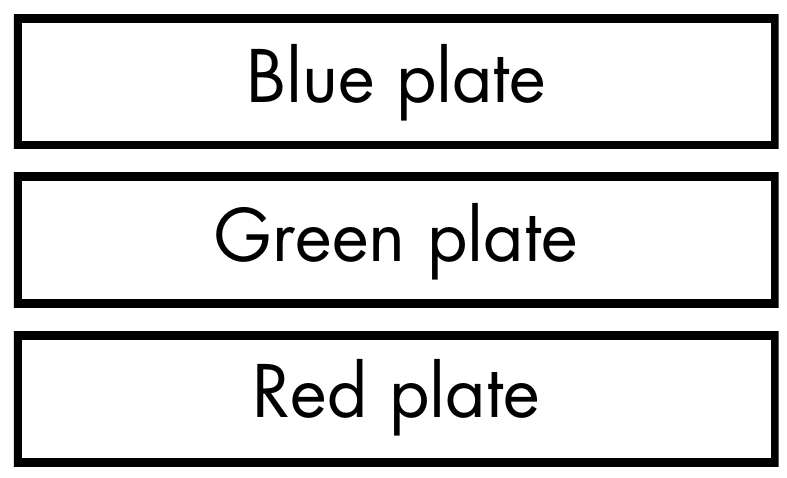
\includegraphics[width=0.5\textwidth]{img/fig11-1.png}
    \caption{Три обеденные тарелки в стопке}
    \label{fig11-1}
\end{figure}

4. Теперь проделайте операцию: вскройте кухонный прилавок. У нас будет синяя тарелка на кухонном столе (напомним, что синяя тарелка стояла на прикроватной тумбочке), а стопка обеденных тарелок останется такой, как показано на рисунке~\ref{fig11-2}.

\begin{figure}[htbp]
    \centering
    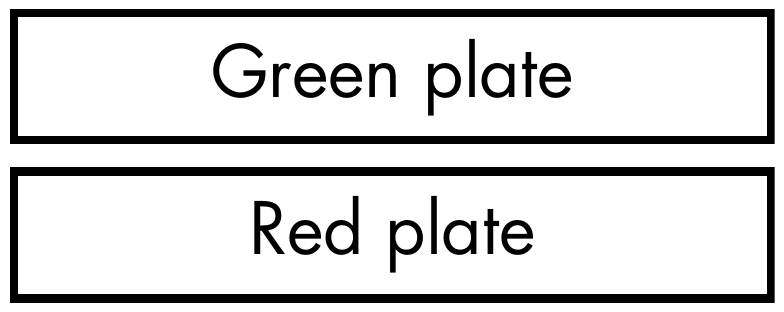
\includegraphics[width=0.5\textwidth]{img/fig11-2.png}
    \caption{Одна тарелка извлечена из стопки}
    \label{fig11-2}
\end{figure}

Если вы догадались, что действительно легко испортить стек, вы правы. Стек должен использоваться в соответствии со строгой дисциплиной. В любой функции:

\begin{itemize}
    \item Всегда помещайте элемент в стек, прежде чем что-либо извлекать.
    \item Никогда не высовывайте больше вещей, чем вы надели.
    \item Всегда выталкивайте все из стека.
\end{itemize}

Если вам не нужно извлекать элементы, вы можете просто настроить указатель стека. Это эквивалентно отбрасыванию элементов, которые выскочили. (Наша аналогия с обеденной тарелкой здесь не работает.)

Хороший способ поддерживать эту дисциплину — подумать об использовании скобок в алгебраическом выражении. Толчок аналогичен левой скобке, а всплывающий аналогичен правой скобке. Пары скобок могут быть вложены друг в друга, но они должны совпадать. Попытка поместить слишком много элементов в стек называется переполнением стека. Попытка вытолкнуть элементы из стека за пределы дна называется недостаточным заполнением стека.

Здесь мы рассмотрели только основные операции со стеком. Обычно в реализации стека добавляются другие операции. Например, операция просмотра позволяет просмотреть элемент на вершине стека, не удаляя его. И, как вы увидите в последующих главах, доступ к элементам, не находящимся на вершине стека, часто осуществляется напрямую, без добавления и извлечения, но очень хорошо контролируемым образом.

Стек реализуется путем выделения ему непрерывной области основной памяти. Стеки могут расти в любом направлении в памяти, в более высокие адреса или в более низкие. Восходящий стек растет до более высоких адресов, а нисходящий стек растет до более низких адресов. Указатель стека может указывать на верхний элемент в стеке, полный стек, или на место в памяти, где следующий элемент будет помещен в стек, пустой стек. Эти четыре возможные реализации стека показаны на рисунке~\ref{fig11-3} с целыми числами 1, 2 и 3, помещенными в стек в указанном порядке. Обязательно обратите внимание, что на этом рисунке адреса памяти увеличиваются вниз, как мы обычно видим их в отладчике \code{gdb}.

\begin{figure}[htbp]
    \centering
    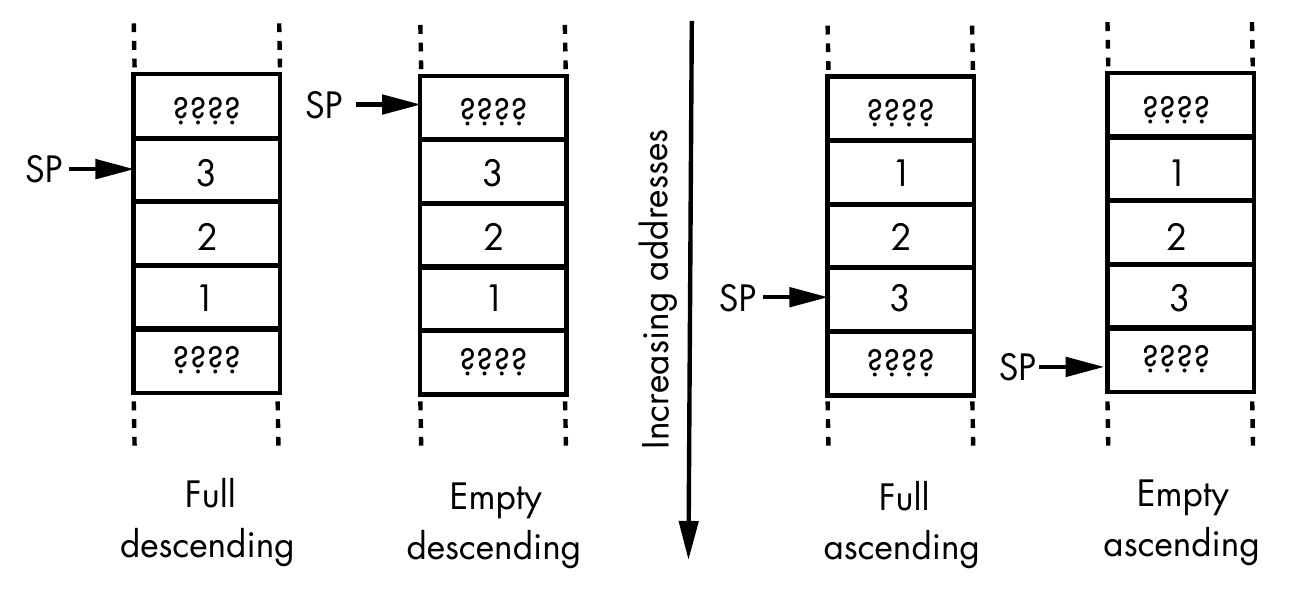
\includegraphics[width=0.9\textwidth]{img/fig11-3.png}
    \caption{Четыре способа реализации стека}
    \label{fig11-3}
\end{figure}

Инструкции x86-64 используют стек как полный нисходящий стек. Чтобы понять этот выбор, подумайте о том, как вы могли бы организовать вещи в памяти. Напомним, что блок управления автоматически увеличивает счетчик программ по мере выполнения вашей программы. Программы бывают самых разных размеров, поэтому хранение программных инструкций по низким адресам памяти обеспечивает максимальную гибкость в отношении размера программы.

Стек является динамической структурой. Вы не знаете заранее, сколько места в стеке потребуется той или иной программе во время ее выполнения. Невозможно узнать, сколько места выделить для стека. Вы хотели бы выделить как можно больше места, не допуская при этом его столкновения с инструкциями программы. Решение состоит в том, чтобы начать стек с наивысшего адреса и увеличивать его в сторону более низких адресов.

Это сильно упрощенное объяснение реализации стеков таким образом, чтобы они росли «вниз» в памяти. Организация различных элементов программы в памяти гораздо сложнее, чем простое описание, данное здесь. Но это может помочь вам понять, что есть несколько веских причин для того, что может показаться довольно странной реализацией.

Важным моментом является то, что нам нужно написать наш ассемблер соответствующим образом. Затем мы подробно рассмотрим, как стек используется в прологе и эпилоге функции, и как аргументы другой функции хранятся в регистрах, написав собственное «Hello, World!» программировать непосредственно на ассемблере.

\subsection{Внутри функции пролога и эпилога}

Моя версия на ассемблере «Hello, World!» Программа в листинге 11-3 очень похожа на язык ассемблера, сгенерированный из версии C компилятором в листинге 11-2, но я добавил комментарии и использовал более осмысленную метку для строковой константы. Это должно облегчить понимание того, как программа использует стек и передает аргументы функции записи.

\begin{ffcode}
# helloWorld.s
# Hello World program using the write() system call
        .intel_syntax noprefix
# Useful constant
        .equ    STDOUT, 1
# Constant data       
        .section  .rodata       
message:
        .string "Hello, World!\n"
        .equ    msgLength, .-message-1

# Code
        .text
        .globl  main
        .type   main, @function
main:
        push    rbp                 # save caller's frame pointer
        mov     rbp, rsp            # our frame pointer

        mov     edx, msgLength      # message length       
        lea     rsi, message[rip]   # message address
        mov     edi, STDOUT         # the screen
        call    write@plt           # write message

        mov     eax, 0              # return 0

        pop     rbp                 # restore caller frame pointer
        ret                         # back to caller
\end{ffcode}

\begin{center}
Листинг 11-3: «Привет, мир!» программа написана на ассемблере
\end{center}

Прежде чем мы перейдем к обсуждению пролога, обратите внимание, что я использовал другую директиву ассемблера, .equ, в листинге 11.3. (1). Формат следующий:

\begin{ffcode}
.equ symbol, expression
\end{ffcode}

Обратите внимание, что нам не нужно указывать сегмент .text для раздела .rodata (2). Ассемблер и компоновщик создают раздел .rodata, и операционная система сама определяет, куда его загрузить.

Выражение должно оцениваться как целое число, и ассемблер устанавливает символ, равный этому значению. Затем вы можете использовать этот символ в своем коде, что значительно облегчит его чтение, а ассемблер подставит значение выражения. Выражение часто представляет собой просто целое число. В этой программе я приравнял символ \code{STDOUT} к целому числу 1.

Cимвол <<\code{.}>> в выражении означает здесь место в памяти. Таким образом, когда ассемблер достигает выражения (3), он вычисляет текущую позицию в памяти, которая является концом текстовой строки в стиле C; вычитает начальное местоположение строки, место, которое программист пометил как сообщение, а затем вычитает 1 для завершающего символа NUL. Конечным результатом является то, что MsgLength приравнивается к количеству печатных символов в текстовой строке.

В главе 10 вы узнали, как указатель фрейма вызывающего объекта сохраняется в стеке вызовов и для этой функции устанавливается новый указатель фрейма. Но теперь, когда вы знаете больше о том, как работает стек вызовов, давайте пройдемся по прологу этой функции с помощью \code{gdb}.

Первое, что нам нужно сделать, это установить точку останова в начале функции:

\begin{ffcode}
    (gdb) b main
    Breakpoint 1 at 0x1139: file helloWorld.s, line 18.
\end{ffcode}

Вы можете использовать либо метку, либо основной, либо номер строки. Мы видели, как использовать команду \code{li} для просмотра номеров строк в главе 2. Использование номера строки может привести к тому, что \code{gdb} выполнит пролог и прекратит работу после него. (Я видел разное поведение в разных версиях \code{gdb}.)

После установки точки останова, когда мы запускаем программу, она прерывается на первой инструкции, и мы можем проверить содержимое регистров \code{rbp} и \code{rsp}:

\begin{ffcode}
    (gdb) r
    Starting program: /home/bob/progs/chap11/helloWorld_asm/helloWorld

    Breakpoint 1, main () at helloWorld.s:18
    18  push  rbp  # save caller's frame pointer
    (gdb) i r rbp rsp
    rbp  0x0  0x0
    rsp  0x7fffffffde88  0x7fffffffde88
\end{ffcode}

Команда \code{i r} дает нам текущее местоположение указателя стека, \code{rsp}. Инструкция, которая должна быть выполнена, поместит восемь байтов регистра \code{rbp} в стек вызовов. Чтобы увидеть эффекты в памяти, мы исследуем текущее содержимое стека. Поскольку стек вызовов полностью нисходящий, мы вычтем 8 из текущего адреса в указателе стека для нашего дисплея, чтобы мы могли получить представление об области памяти, которую эта инструкция изменит до того, как она изменится:

\begin{ffcode}
    (gdb) x/2xg 0x7fffffffde80
    0x7fffffffde80: 0x0000555555555160  0x00007ffff7de70b3
\end{ffcode}

Указатель стека в настоящее время указывает на значение 0x00007ffff7de70b3, которое является адресом возврата, который инструкция вызова в вызывающей функции (в среде выполнения C, поскольку это основная функция) помещается в стек. Регистр \code{rbp} содержит 0x0000000000000000. Это значение будет помещено в стек по адресу 0x7ffffffffde80, который в настоящее время содержит 0x00005555555555160.

Затем мы выполняем две инструкции в прологе функции, что приведет нас к первой инструкции после пролога:

\begin{ffcode}
    (gdb) si
    19  mov  rbp, rsp  # our frame pointer
    (gdb) si
    21  mov  edx, MsgLength  # message length
\end{ffcode}

Мы проверим значения в регистрах rsp и rbp:

\begin{ffcode}
    (gdb) i r rbp rsp
    rbp  0x7fffffffde80  0x7fffffffde80
    rsp  0x7fffffffde80  0x7fffffffde80
\end{ffcode}

...

\section{Локальные переменные в функции}

Переменные, определенные в функции C, могут использоваться в функции только там, где они определены, что делает их локальными переменными. Они создаются при вызове функции и удаляются, когда функция возвращается к вызывающей функции, поэтому их также называют автоматическими переменными.

В главе 9 вы узнали, что регистры ЦП можно использовать в качестве переменных, но если бы мы использовали регистры ЦП для хранения всех наших переменных, у нас скоро закончились бы регистры даже в небольшой программе, поэтому нам нужно выделить место в память для переменных.

Ранее мы также видели, что функция должна сохранять содержимое некоторых регистров (столбец «Сохранить?» в таблице 11.2) для вызывающей функции. Если мы хотим использовать такой регистр в нашей функции, нам нужно сохранить его содержимое в памяти и восстановить перед возвратом в вызывающую функцию.

Далее мы рассмотрим, как использовать стек вызовов для этих двух целей: создание и удаление автоматических переменных и сохранение и восстановление содержимого регистров.

\subsection{Переменные в стеке}

Из описания стека вызовов, показанного ранее, вы можете догадаться, что это хорошее место для сохранения содержимого регистра — просто поместите его в стек, прежде чем использовать регистр для чего-то другого, а затем извлеките содержимое из регистра перед возвратом в регистр. вызывающая функция.

Создание переменных в стеке вызовов более сложно. Если мы ограничим наше использование стека отправкой и извлечением, отслеживание того, где находится каждая переменная в стеке, быстро станет беспорядочной, если не невозможной.

Однако есть простой способ использовать стек для переменных. В рамках пролога функции мы выделим достаточно памяти для переменных в стеке, переместив указатель стека, тем самым увеличив размер кадра стека для функции. Мы можем использовать тот же метод адресации для доступа к нашим переменным в кадре стека, который использовался для доступа к адресу сообщения в листинге 11-3, за исключением того, что мы будем использовать указатель кадра, \code{rbp}, для базы адреса. Мы должны быть осторожны, чтобы не изменить \code{rbp}, чтобы мы могли использовать его в качестве контрольной точки во фрейме стека, оставляя указатель стека свободным для добавления и извлечения элементов по мере необходимости.

Чтобы проиллюстрировать, как использовать кадр стека для автоматических локальных переменных, мы начнем с программы на C в листинге 11.4, которая считывает один символ с клавиатуры и выводит его на экран.

\begin{ffcode}
/* echoChar.c
 * Echoes a character entered by the user.
 */

#include <unistd.h>

int main(void)
{
  char aLetter;

  write(STDOUT_FILENO, "Enter one character: ", 21); /* prompt user   */
  read(STDIN_FILENO, &aLetter, 1);                   /* one character */
  write(STDOUT_FILENO, "You entered: ", 13);         /* message       */
  write(STDOUT_FILENO, &aLetter, 1);

  return 0;
}
\end{ffcode}

\begin{center}
Листинг 11-4: Программа для отображения одного символа, введенного пользователем    
\end{center}


В листинге 11-5 показано, как это делает наш компилятор, представляющий собой язык ассемблера, который gcc генерирует для программы C в листинге 11-4.

\begin{ffcode}
	.file	"echoChar.c"
	.intel_syntax noprefix
	.text
	.section	.rodata
.LC0:
	.string	"Enter one character: "
.LC1:
	.string	"You entered: "
	.text
	.globl	main
	.type	main, @function
main:
	push	rbp
	mov	rbp, rsp
	sub	rsp, 16
	mov	rax, QWORD PTR fs:40
	mov	QWORD PTR -8[rbp], rax
	xor	eax, eax
	mov	edx, 21
	lea	rax, .LC0[rip]
	mov	rsi, rax
	mov	edi, 1
	call	write@PLT
	lea	rax, -9[rbp]
	mov	edx, 1
	mov	rsi, rax
	mov	edi, 0
	call	read@PLT
	mov	edx, 13
	lea	rax, .LC1[rip]
	mov	rsi, rax
	mov	edi, 1
	call	write@PLT
	lea	rax, -9[rbp]
	mov	edx, 1
	mov	rsi, rax
	mov	edi, 1
	call	write@PLT
	mov	eax, 0
	mov	rdx, QWORD PTR -8[rbp]
	sub	rdx, QWORD PTR fs:40
	je	.L3
	call	__stack_chk_fail@PLT
.L3:
	leave
	ret
	.size	main, .-main
	.ident	"GCC: (GNU) 12.1.1 20220730"
	.section	.note.GNU-stack,"",@progbits
\end{ffcode}

\begin{center}
Листинг 11-5. Язык ассемблера, сгенерированный компилятором для программы echoChar в листинге 11-4.
\end{center}

Программа на C определяет локальную символьную переменную \code{aLetter}, которая требует только один байт. Однако компилятор выделил 16 байтов в стеке вызовов, просто переместив указатель стека на 1. Архитектура x86-64 включает набор из шестнадцати 128-битных регистров, которые используются некоторыми инструкциями с плавающей запятой и векторами. Вы узнаете о них больше в главе 18. Для этих инструкций указатель стека должен быть выровнен по 16-байтовым границам адреса, поэтому в большинстве стандартов протоколов указано, что указатель стека должен быть выровнен по 16-байтовым границам. Это менее подвержено ошибкам, чем выравнивание указателя стека только там, где это необходимо.

Инструкция по перемещению указателя стека вводит инструкцию вычитания \code{sub}. Пока мы здесь, мы также опишем инструкции сложения и отрицания, сложения и отрицания.

...

Инструкции по умножению и делению более сложны и описаны в главе 16.

Нам нужно передать адрес локальной переменной \code{char} функции чтения, чтобы она могла сохранить там символ, введенный пользователем. Мы можем сделать это с помощью инструкции \code{lea} (загрузить эффективный адрес) (4). Как видите, компилятор выбрал байт, расположенный в 9 байтах внутри 16 байтов, выделенных в стеке. На рисунке~\ref{fig11-4} показано расположение этой переменной.

\begin{figure}[htbp]
    \centering
    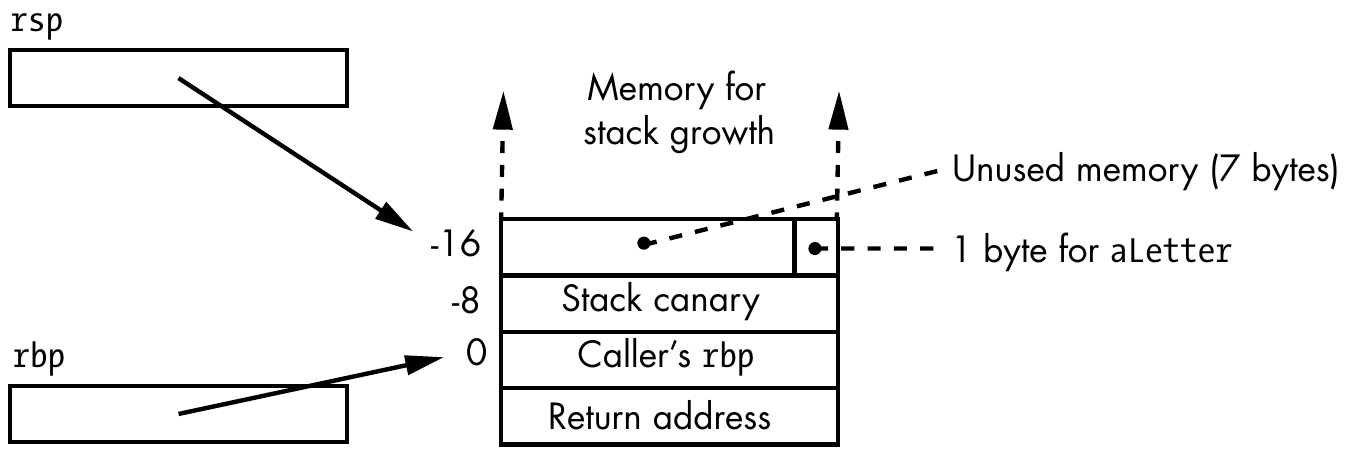
\includegraphics[width=0.9\textwidth]{img/fig11-4.png}
    \caption{Фрейм стека для программы в листинге 11-5}
    \label{fig11-4}
\end{figure}


Один из элементов кадра стека на рисунке~\ref{fig11-4} — это канарейка стека, которая используется для обнаружения повреждения стека.

\subsection{Повреждение стека}

Эпилог функции восстанавливает указатель фрейма вызывающего объекта в регистре rbp и возвращает указатель стека, указывающий на адрес возврата. Однако, если любое из этих значений было изменено в стеке, программа не будет вести себя должным образом. Канарейка стека может помочь определить, было ли изменено какое-либо из этих значений.

Когда программа запускается, операционная система сохраняет 64-битное случайное число в специальном месте памяти с пометкой \code{fs:40}, которое может изменить только операционная система. Мы читаем это значение из памяти (2) и сохраняем его во фрейме стека сразу после значения \code{rbp} (3) вызывающей программы. Затем, перед выполнением эпилога функции, мы проверяем, не изменилось ли значение стековой канарейки (5).

\textbf{Примечание.}
\textit{Использование стековой канарейки — необязательная функция. В моей версии \code{gcc} он используется по умолчанию. Вы можете переопределить поведение по умолчанию с помощью одного из параметров командной строки \code{-fstack-protector}, \code{-fstack-protector-strong} или \\ \code{-stack-protector-all}, чтобы использовать канарейку стека, и\\ \code{-fno-stack-protector}, чтобы не использовать ее.}

Код для выполнения этой проверки содержит еще две инструкции.

...

В листинге 11-5 код для проверки поврежденного стека 5 сначала извлекает значение, которое было сохранено в стеке, канареечный стек, а затем выполняет побитовое исключающее ИЛИ с исходным значением, которое было сгенерировано при первом запуске программы. в ячейке памяти \code{fs:40}. Если эти два значения идентичны, исключающее ИЛИ приводит к 0, что устанавливает флаг нулевого состояния \code{ZF} в 1 (истина), в результате чего инструкция \code{je .L3} переводит поток программы на инструкцию выхода, пропуская, таким образом, вызов функция \verb|__stack_chk_fail@PLT|. Если операция исключающее ИЛИ не возвращает 0, переход не произойдет, и программа вызовет функцию \verb|__stack_chk_fail@PLT|, которая сообщит об ошибке повреждения стека и завершит программу.

Вы видите еще одну новую инструкцию в этой программе, уходите.

...

Язык ассемблера, сгенерированный gcc в листинге 11.5, включает некоторые дополнительные обозначения \code{QWORD PTR 25}. В большинстве случаев ассемблер может вычислить размер операнда — байта, слова, двойного слова или четверного слова — из контекста инструкция. Если один из операндов является регистром, имя регистра определяет размер операнда. Но если один из операндов является адресом памяти, а другой — буквальной константой, размер операнда определить невозможно. Например, в листинге 11-5, если бы инструкция в 3 была следующей:

...

Давайте соберем все это воедино и напишем программу \code{echoChar} непосредственно на ассемблере. Мы будем использовать более осмысленные имена для меток, позволим ассемблеру вычислить длину текстовых строк и прокомментируем наш код, как показано в листинге 11.6.

\begin{ffcode}
# echoChar.s
# Prompts user to enter a character, then echoes the response
        .intel_syntax noprefix
# Useful constants
        .equ    STDIN,0
        .equ    STDOUT,1
# Stack frame
        .equ    aLetter,-9
        .equ    canary,-8
        .equ    localSize,-16

# Constant data
        .section  .rodata
prompt:
        .string "Enter one character: "
        .equ    promptSz,.-prompt-1
msg:
        .string "You entered: "
        .equ    msgSz,.-msg-1
        .text
# Code 
        .globl  main
        .type   main, @function
main:
        push    rbp                   # save caller's frame pointer
        mov     rbp, rsp              # our frame pointer
        add     rsp, localSize        # for local var.

        mov     rax, fs:40            # get stack canary
        mov     canary[rbp], rax      # and save it

        mov     edx, promptSz         # prompt size
        lea     rsi, prompt[rip]      # address of prompt text string
        mov     edi, STDOUT           # standard out
        call    write@plt             # invoke write function

        mov     edx, 1                # 1 character
        lea     rsi, aLetter[rbp]     # place to store character
        mov     edi, STDIN            # standard in
        call    read@plt              # invoke read function

        mov     edx, msgSz            # message size
        lea     rsi, msg[rip]         # address of message text string
        mov     edi, STDOUT           # standard out
        call    write@plt             # invoke write function

        mov     edx, 1                # 1 character
        lea     rsi, aLetter[rbp]     # place where character stored
        mov     edi, STDOUT           # standard out
        call    write@plt             # invoke write function

        mov     eax, 0                # return 0

        mov     rcx, canary[rbp]      # retrieve saved canary
        xor     rcx, fs:40            # and check it
        je      goodCanary
        call    __stack_chk_fail@PLT  # bad canary
goodCanary:
        mov     rsp, rbp              # delete local variables
        pop     rbp                   # restore caller's frame pointer
        ret                           # back to calling function
\end{ffcode}

\begin{center}
Листинг 11-6: Программа для отображения одного символа, написанная непосредственно на ассемблере
\end{center}

Читая код в листинге 11-6, я думаю, вы обнаружите, что присвоение имен смещениям для переменных в кадре стека значительно упрощает чтение кода. (1). Я также явно отменяю кадр стека вместо использования инструкции выхода. подчеркнуть происходящее (2).

В последующих главах вы узнаете, как использовать фрейм стека для более крупных и сложных переменных. Вы также узнаете, как использовать стек для передачи аргументов помимо шести, которые могут быть переданы в регистрах.

\section{Не использовать среду выполнения C}

Основная цель этой книги — показать, что происходит на уровне набора инструкций при написании на языках высокого уровня, поэтому мы продолжим использовать среду выполнения C (а позже и C++) и системный вызов записи и чтения POSIX. функции для оставшейся части этой книги.

Конечно, можно писать автономные программы, не использующие среду выполнения C. Вы увидите, как это делается, в главе 20.

...

% --- Заключене -------------------------------------------
\chapter*{Заключение}
\addcontentsline{toc}{chapter}{Заключение}

%\centering
\framebox[0.8\textwidth][l]{\textit{Продолжение следует...}}


% --- Библиография -------------------------------------------
\begin{thebibliography}{00}
%\addcontentsline{toc}{section}{Литература}

\bibitem
{risc-v}
RISC-V International. Описание архитектуры и ее обоснование.
--- \url{https://riscv.org/}

\bibitem
{Harris}
Сара Л. Харрис, Дэвид Харрис.
Цифровая схемотехника и архитектура компьютера: RISC-V / пер. с англ. В. С. Яценкова, А. Ю. Романова; под ред. А. Ю. Романова. --- М.: ДМК Пресс, 2021. --- 810 с.

\bibitem
{Borin}
Edson Borin
An Introduction to Assembly Programming with RISC-V /
Document version: May 9, 2022
--- \url{https://riscv-programming.org/}


\bibitem
{kur-2022}
Курячий Георгий. Архитектура и язык ассемблера RISC-V. Весна 2022.
--- \url{http://uneex.ru/LecturesCMC/ArchitectureAssembler2022}

\bibitem
{aps-git}
Семестровый забег "Архитектур процессорных систем"
--- \url{https://github.com/MPSU/APS}

\bibitem
{kur-youtube-2022}
[UNИX] Архитектура и язык ассемблера RISC-V. Видео лекции. Весна 2022.
--- \url{https://www.youtube.com/playlist?list=PL6kSdcHYB3x6cjkby4H1RuRMzfbEGSNBi}

\bibitem
{aps-youtube}
Архитектуры процессорных систем
--- \url{https://www.youtube.com/c/%D0%90%D0%9F%D0%A1%D0%9F%D0%BE%D0%BF%D0%BE%D0%B2}

\bibitem
{RARS}
RARS -- RISC-V Assembler and Runtime Simulator
--- \url{https://github.com/TheThirdOne/rars}

\bibitem
{Ripes}
Ripes. A visual computer architecture simulator and assembly code editor.
--- \url{https://github.com/mortbopet/Ripes}

\bibitem
{QtRvSim}
QtRvSim–RISC-V CPU simulator for education
--- \url{https://github.com/cvut/qtrvsim}

\bibitem
{Goossens}
Goossens Bernard.
Guide to Computer Processor Architecture. A RISC-V Approach, with High-Level Synthesis.
--- Springer Nature. Switzerland AG --- 2023.

\bibitem
{Booch92}
Буч Г.
Объектно-ориентированное проектирование с примерами применения. /Пер. с англ.
--- М.: Конкорд, 1992. --- 519 с.

\bibitem
{Gay}
Gay Warren.
RISC-V Assembly Language Programming. Using ESP32-C3 and QEMU.
--- Elektor International Media B.V. --- 2022.

\bibitem
{Booch98}
Буч Г.
Объектно-ориентированный анализ и проектирование с примерами приложений на C++, 2-е изд./Пер. с англ.
--- М.: «Издательства Бином», СПб: «Невский диалект», 1998 г. --- 560 с., ил.

\bibitem
{ERD-dict}
Англо-русско-немецко-французский толковый словарь по вычислительной технике и обработке данных, 4132 термина.
Под. ред. А.А. Дородницына. М.: 1978. --- 416 с.

\bibitem
{Gagarina}
Гагарина Л.Г., Кононова А.И.
Архитектура вычислительных систем и Ассемблер с приложением методических указаний к лабораторным работам. Учебное пособие.
--- М.: СОЛОН-Пресс, 2019. --- 368 с.

\bibitem
{elf64}
Формат файла ELF64.
--- \url{https://uclibc.org/docs/elf-64-gen.pdf}

\bibitem
{Plantz}
Plantz Robert G.
Introduction to Computer Organization.
--- 2022

\bibitem
{gdb-stollman}
Ричард Столмен, Роланд Пеш, Стан Шебс и др.
Отладка с помощью GDB.
--- 2000

\bibitem
{gdb-zeller}
Андреас Целлер
Почему не работают программы.
--- М.: Эксмо, 2011. --- 560 с.

\bibitem
{gdb-dive-into-systems}
Suzanne J. Matthews, Tia Newhall, Kevin C. Webb.
Dive into Systems.
--- 2022

\bibitem
{round-up}
Округление. Статья в Википедии.
--- \url{https://ru.wikipedia.org/wiki/%D0%9E%D0%BA%D1%80%D1%83%D0%B3%D0%BB%D0%B5%D0%BD%D0%B8%D0%B5}

\bibitem
{c-lang}
Прохоренок Н.А.
Язык С. Самое необходимое.
--- СПб.: БХВ-Петербург, 2020. --- 480 с.

\bibitem
{nasm-x64}
Йо Ван Гуй.
Программирование на ассемблере x64: от начального уровня до профессионального использования AVX.
--- М.: ДМК Пресс, 2021. --- 332 с.

\bibitem
{wsl}
Установка Linux на Windows с помощью WSL
--- \url{https://docs.microsoft.com/ru-ru/windows/wsl/install}

\bibitem
{vir-box}
Установка Linux на Virtualbox.
--- \url{https://losst.ru/ustanovka-linux-na-virtualbox}

\bibitem
{System-V}
System V Application Binary Interface AMD64 Architecture Processor Supplement (With LP64 and ILP32 Programming Models). Version 1.0. --- 2018.
--- \url{https://github.com/hjl-tools/x86-psABI/wiki/x86-64-psABI-1.0.pdf}



\end{thebibliography}


\end {document}
